\documentclass[10pt]{article}
\usepackage[margin=1in]{geometry}
 \usepackage{auto-pst-pdf}
\usepackage{graphicx}
%\usepackage{arydshln}
\usepackage{ifpdf}
\ifpdf
  \usepackage{epstopdf}
\fi
\usepackage{multirow}
\usepackage{epsfig}
\usepackage{float}
\usepackage{url}
\usepackage{color}
\usepackage{subfigure}

%\newcommand\solidrule[1][1cm]{\rule[0.5ex]{#1}{.4pt}}
%\newcommand\dashedrule{\mbox{%
%  \solidrule[2mm]\hspace{2mm}\solidrule[2mm]\hspace{2mm}\solidrule[2mm]}}
  
%\usepackage{hyperref}

\begin{document}
\title{Machine Homogeneity Check on EMPv5}

\author{
Young-Kyoon Suh\\
}
\maketitle

\section{Experiment Notes}
%% done
\begin{table}[h]
\begin{center}
\begin{tabular}{|p{2cm}|p{3cm}|p{6cm}|p{4cm}|} \hline
Machine & Task Length & Description & Time Length\\ \hline
{\tt sodb8} &  INC1$\sim$INC128 & Runs of 300 samples & 2017-02-09 $\sim$ 2017-02-10\\ \hline
{\tt sodb9} &  INC1$\sim$INC128 & Runs of 300 samples & 2017-02-09 $\sim$ 2017-02-10\\ \hline
{\tt sodb10} & INC1$\sim$INC128 & Runs of 300 samples & 2017-02-09 $\sim$ 2017-02-10\\ \hline
{\tt sodb12} & INC1$\sim$INC128 & Runs of 300 samples & 2017-02-09 $\sim$ 2017-02-10\\ \hline
\end{tabular}
\end{center}
\vspace{-.2in}
\caption{Detailed description of INC data used for histograms\label{tab:exp_notes}}
\end{table}

The following sections presents experimental results on a machine basis. 
We used four nodes in a cluster. 
Each section exhibits histograms of elapsed time (ET) and process time (PT) 
over increasing INC's task lengths on each individual machine. 

%\begin{table}[h]
%\begin{center}
%\begin{tabular}{|l|l|l|l}|} \hline
%Machine & {\tt sodb8} & {\tt sodb9} & {\tt sodb10} & {\tt sodb12} \\ \hline
%1  & \\ \hline
%2  & \\ \hline
%4  & \\ \hline
%8  & \\ \hline
%16 & \\ \hline
%32 & \\ \hline
%64 & \\ \hline
%128 & \\ \hline
%\end{tabular}
%\end{center}
%\caption{Machine-wise Run Statistics: Standard Deviation\label{tab:std_machine}}
%\end{table}

\newpage

\section{{\tt sodb9}~\label{sec:sodb9_hist}} 
This section exhibits histograms on the EMPv5 data obtained on {\tt sodb9}. 
The detailed description of the base data are from Table~\ref{tab:exp_notes}.

\subsection{ET}

\begin{figure}[hp!]
	\centering
	\subfigure[ET frequency on INC1]{
		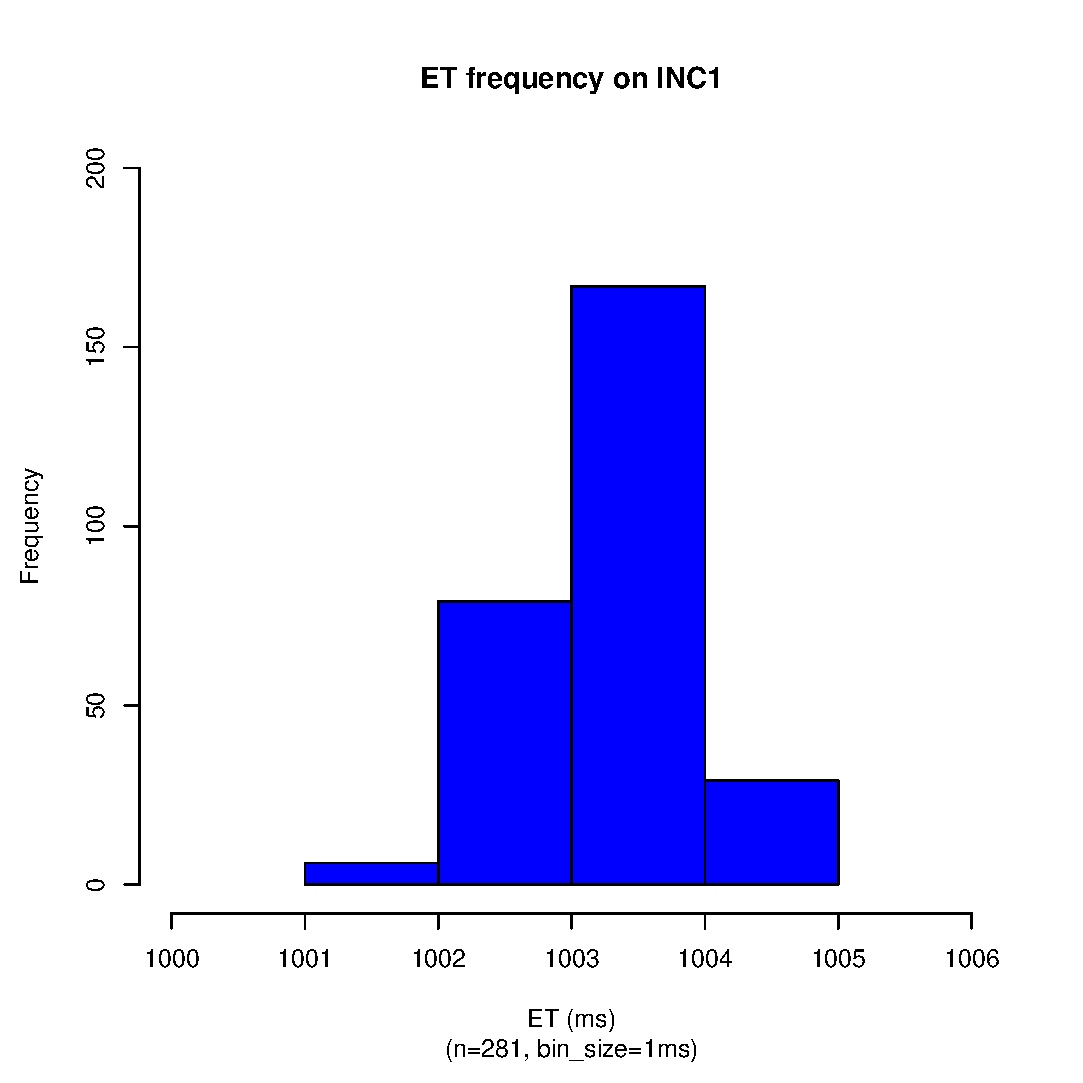
\includegraphics[scale=0.43]{sodb9/1_sec_et_hist_v5.eps}
		\label{fig:inc1_et_hist_v5}
	}
	\subfigure[ET frequency on INC2]{
		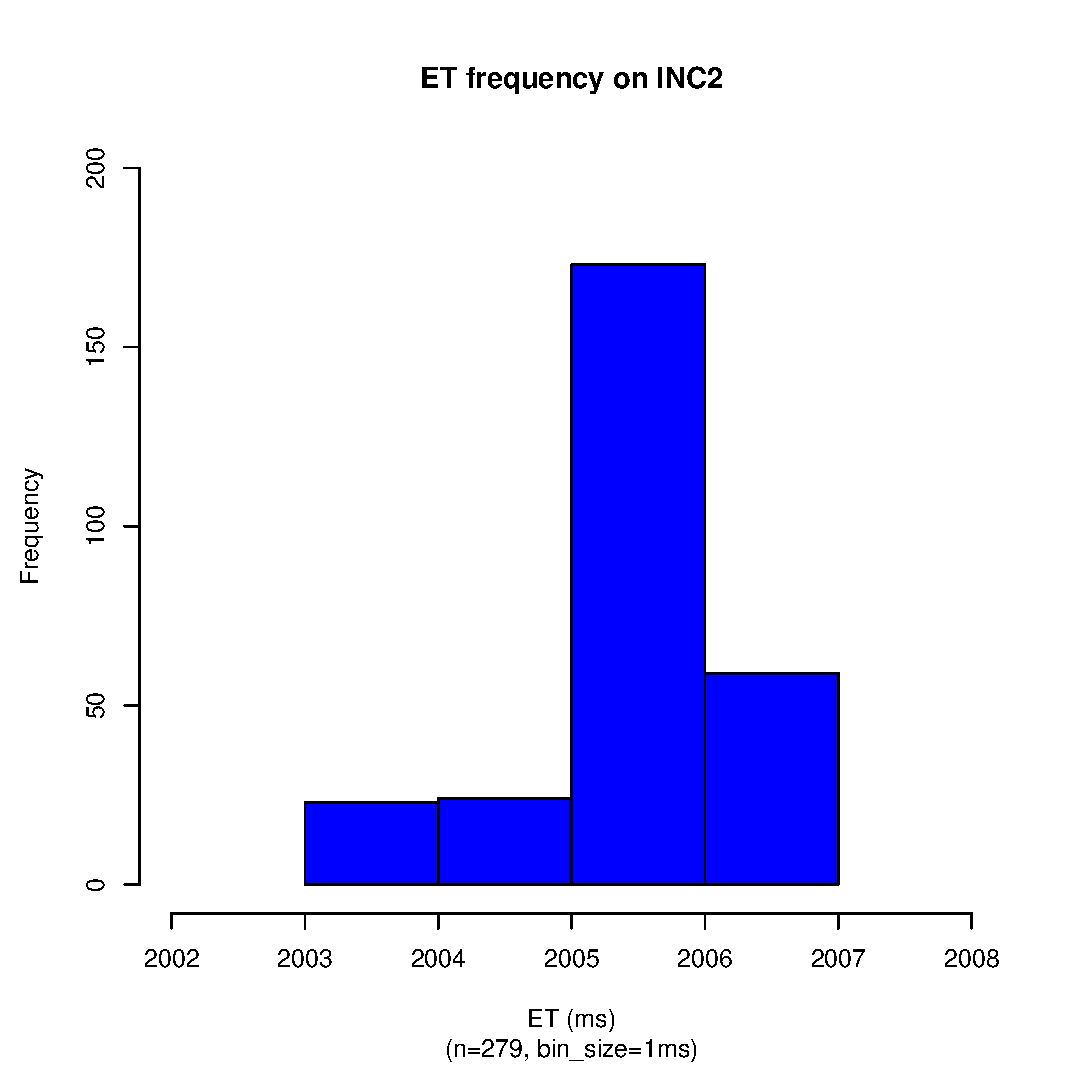
\includegraphics[scale=0.43]{sodb9/2_sec_et_hist_v5.eps}
		\label{fig:inc2_et_hist_v5}
	}
	\subfigure[ET frequency on INC4]{
		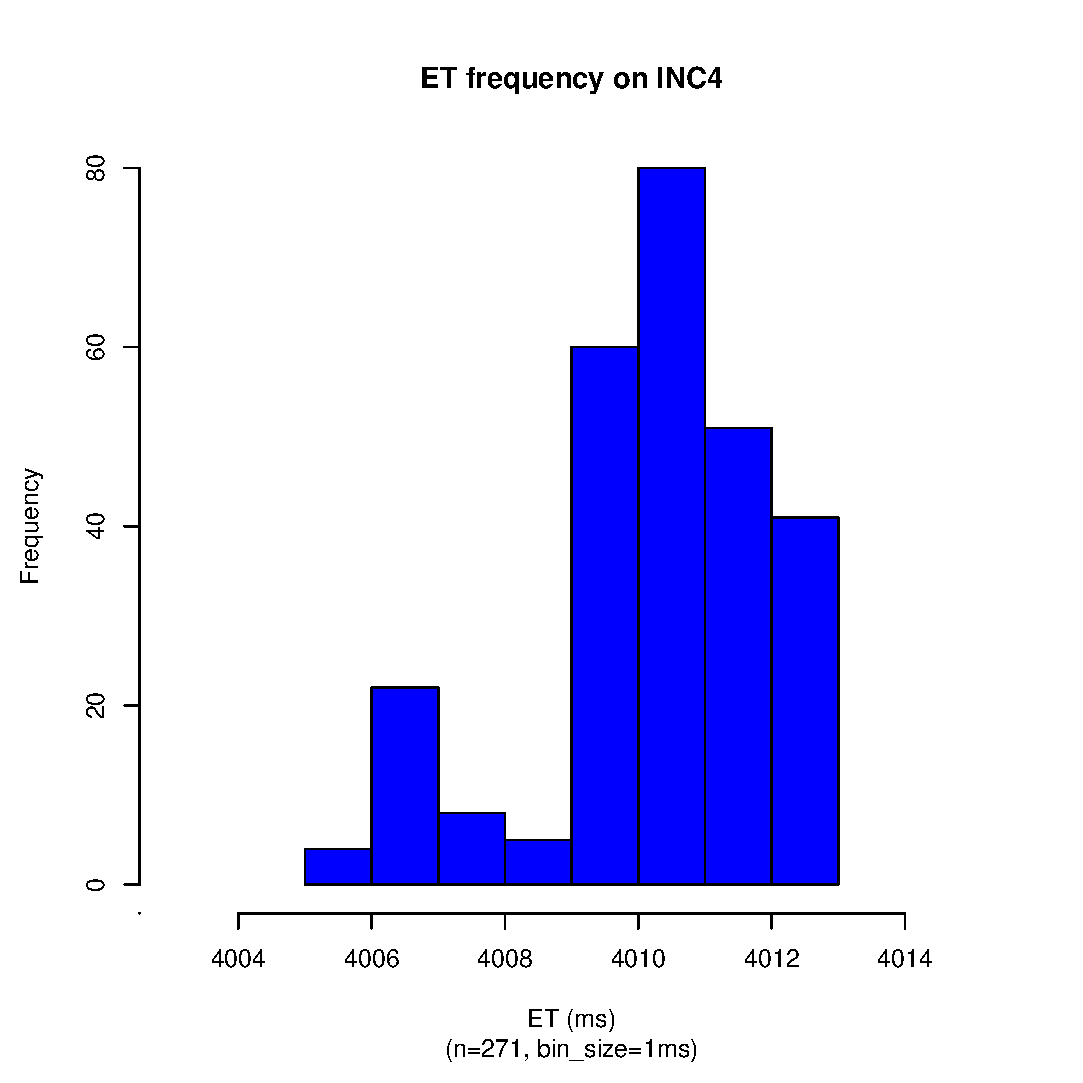
\includegraphics[scale=0.43]{sodb9/4_sec_et_hist_v5.eps}
		\label{fig:inc4_et_hist_v5}
	}
	\subfigure[ET frequency on INC8]{
		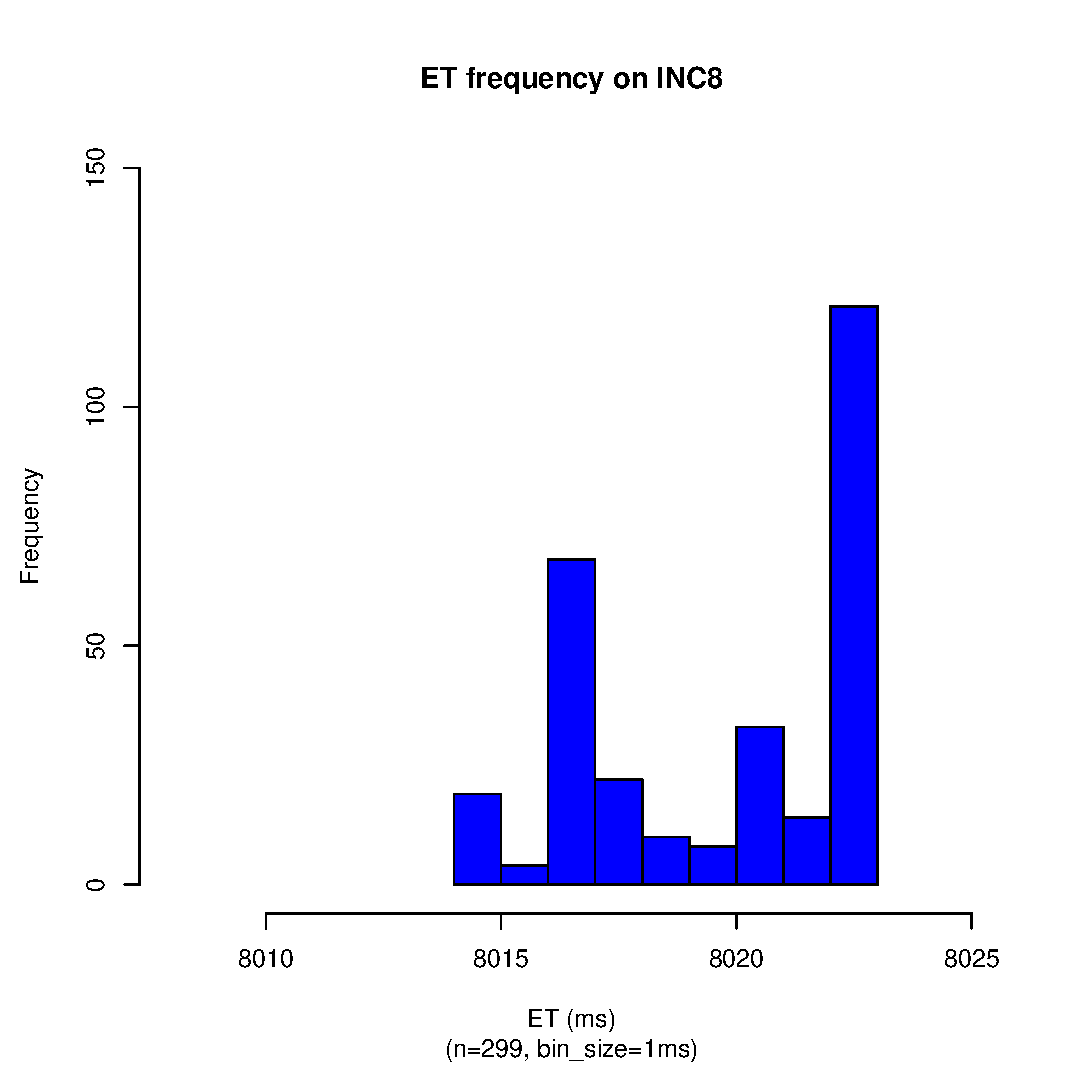
\includegraphics[scale=0.43]{sodb9/8_sec_et_hist_v5.eps}
		\label{fig:inc8_et_hist_v5}
	}
	\caption{ET Histograms of INC1 ... INC8~\label{fig:s9_et_hist1}}
\end{figure}

\begin{figure}[hp!]
	\centering
	\subfigure[ET frequency on INC16]{
		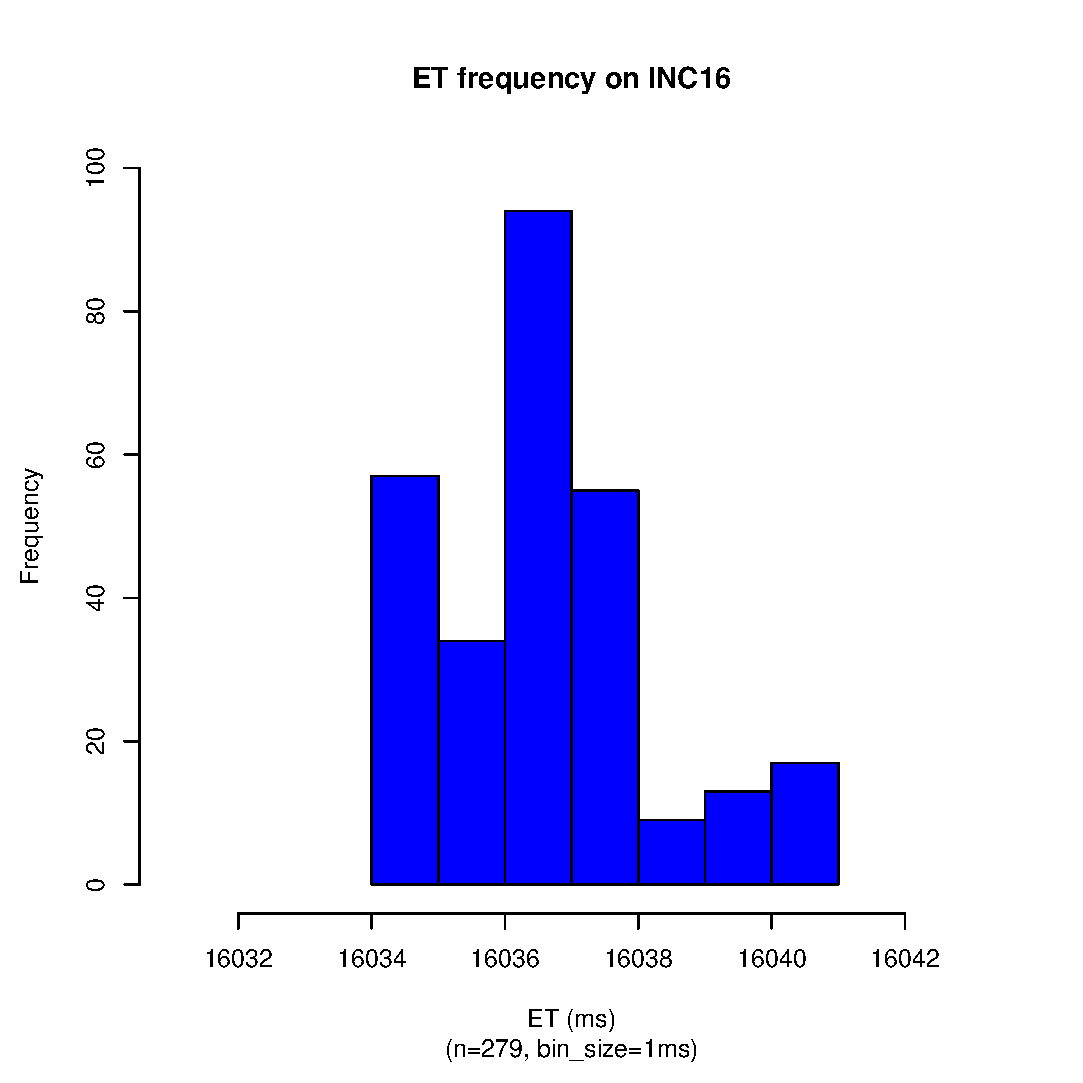
\includegraphics[scale=0.43]{sodb9/16_sec_et_hist_v5.eps}
		\label{fig:inc16_et_hist_v5}
	}
	\subfigure[ET frequency on INC32]{
		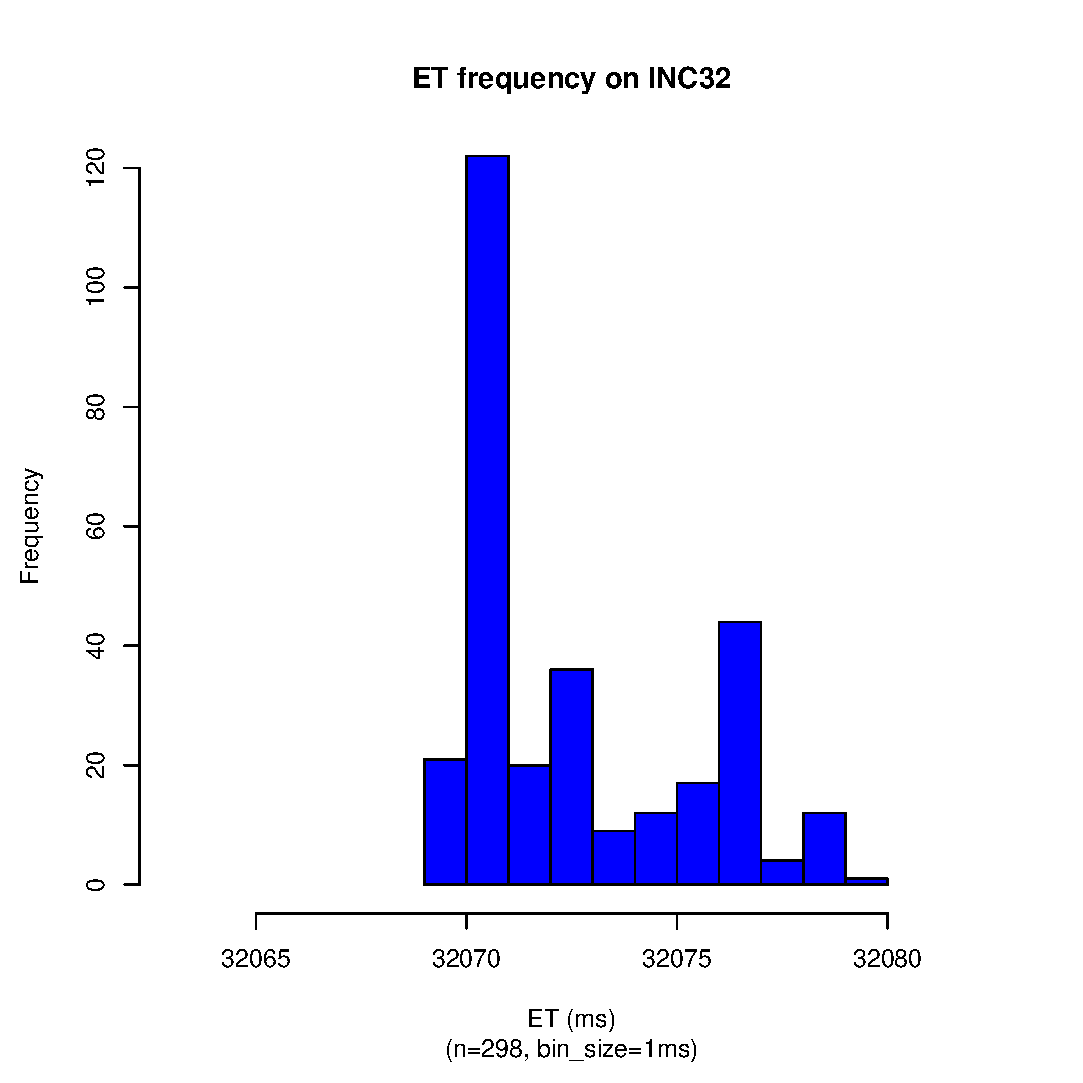
\includegraphics[scale=0.43]{sodb9/32_sec_et_hist_v5.eps}
		\label{fig:inc32_et_hist_v5}
	}
	\subfigure[ET frequency on INC64]{
		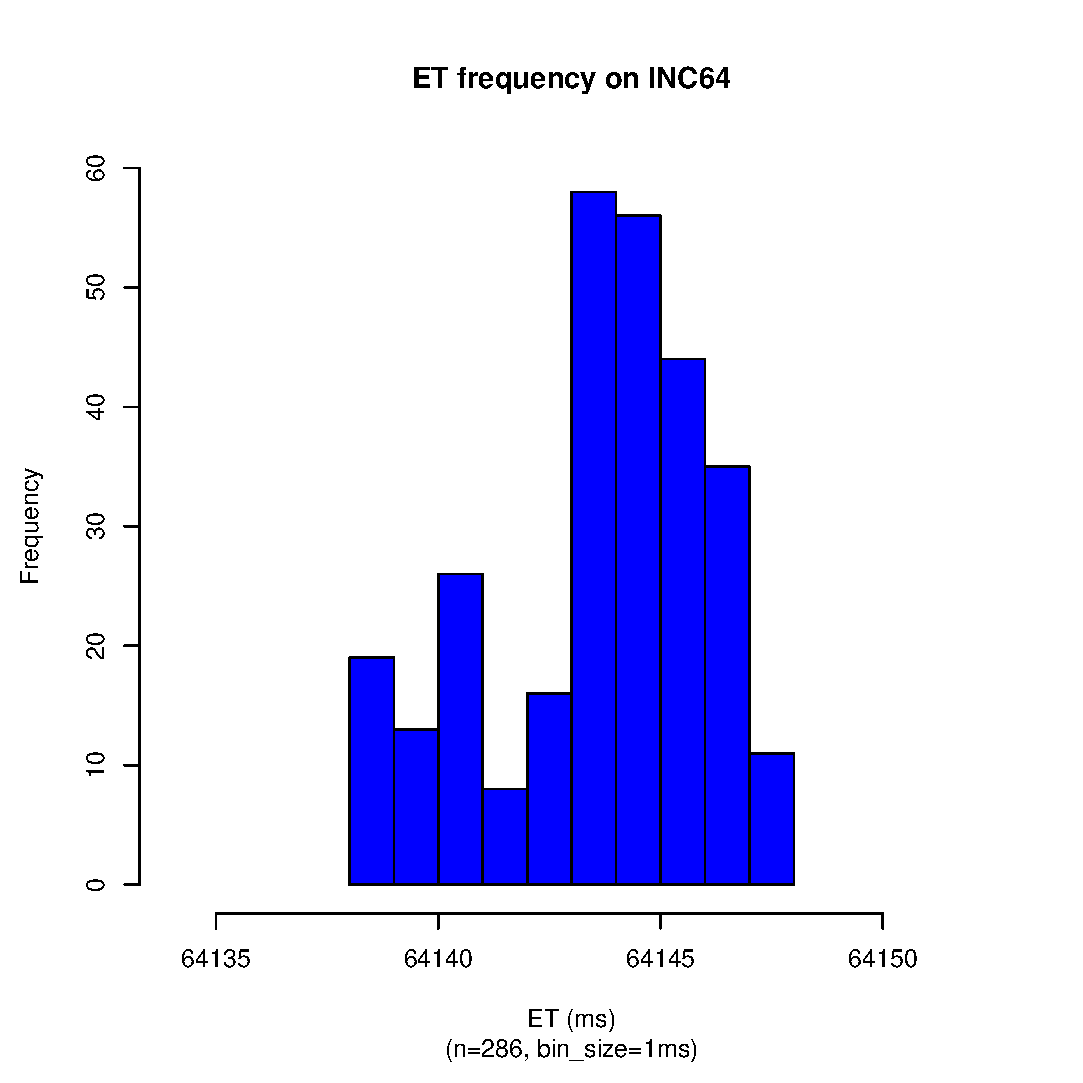
\includegraphics[scale=0.43]{sodb9/64_sec_et_hist_v5.eps}
		\label{fig:inc64_et_hist_v5}
	}
	\subfigure[ET frequency on INC128]{
		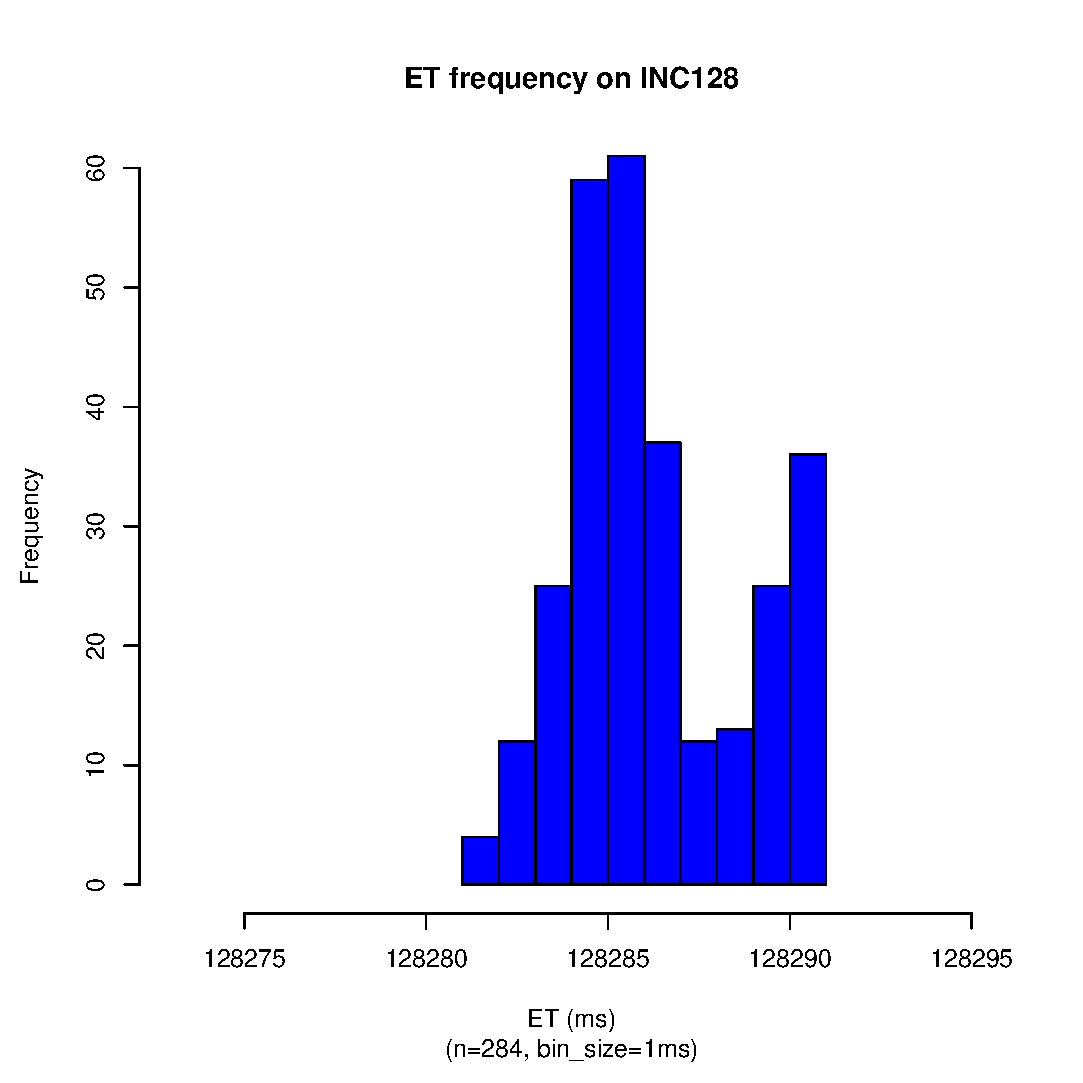
\includegraphics[scale=0.43]{sodb9/128_sec_et_hist_v5.eps}
		\label{fig:inc128_et_hist_v5}
	}
	\caption{ET Histograms of INC16 ... INC128~\label{fig:s9_et_hist2}}
\end{figure}

\newpage

\subsection{PT}

\begin{figure}[hp!]
	\centering
	\subfigure[PT frequency on INC1]{
		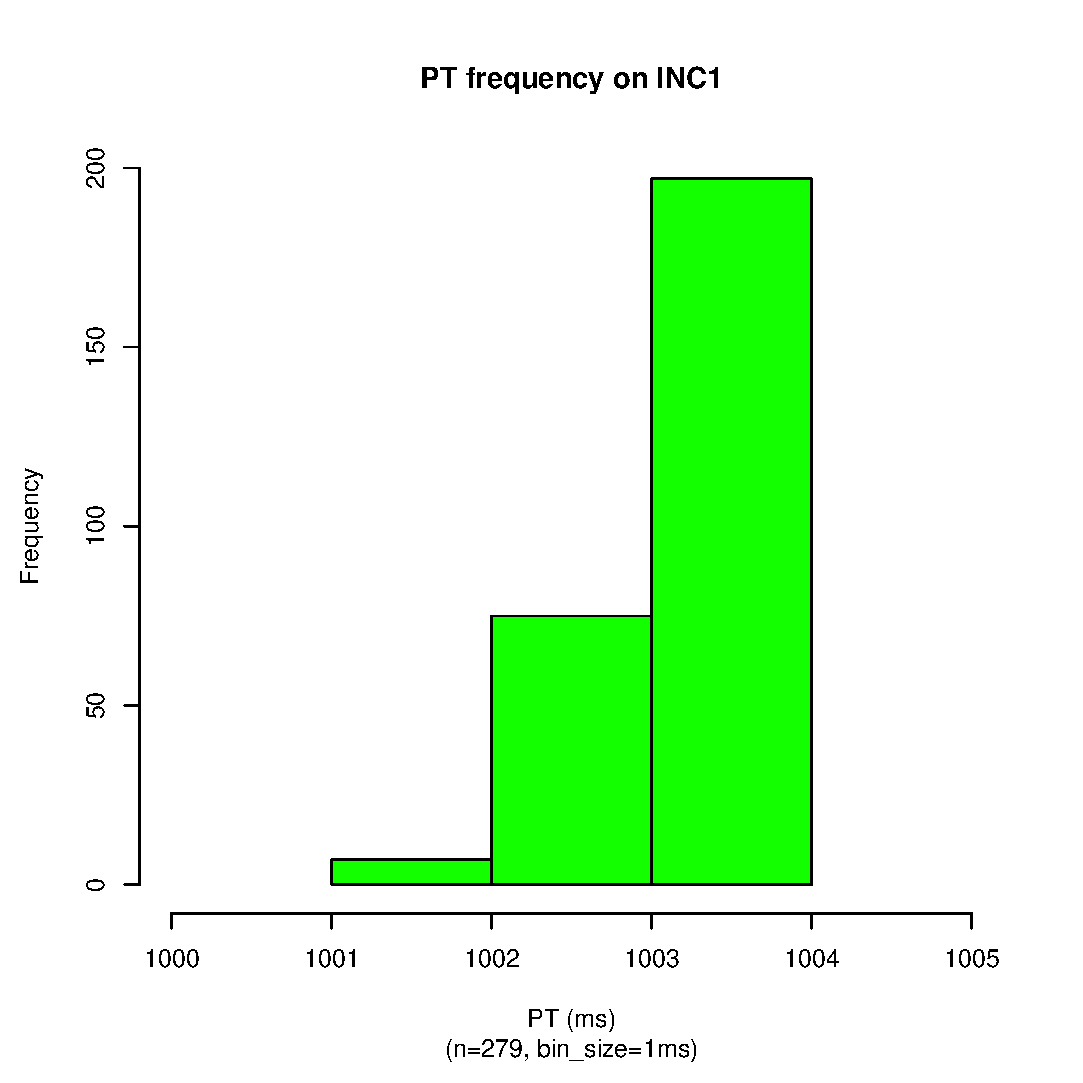
\includegraphics[scale=0.43]{sodb9/1_sec_pt_hist_v5.eps}
		\label{fig:inc1_hist_v5}
	}
	\subfigure[PT frequency on INC2]{
		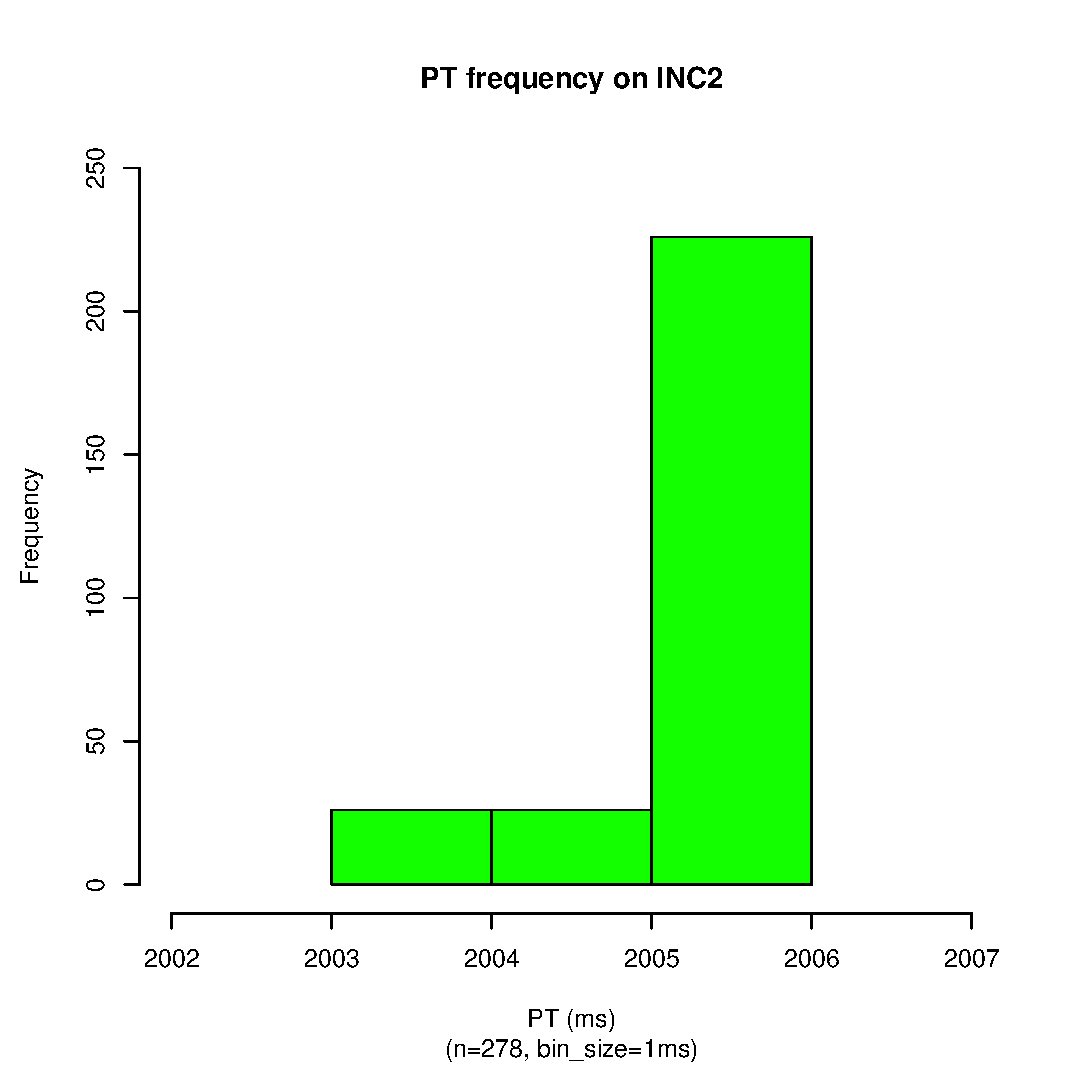
\includegraphics[scale=0.43]{sodb9/2_sec_pt_hist_v5.eps}
		\label{fig:inc2_hist_v5}
	}
	\subfigure[PT frequency on INC4]{
		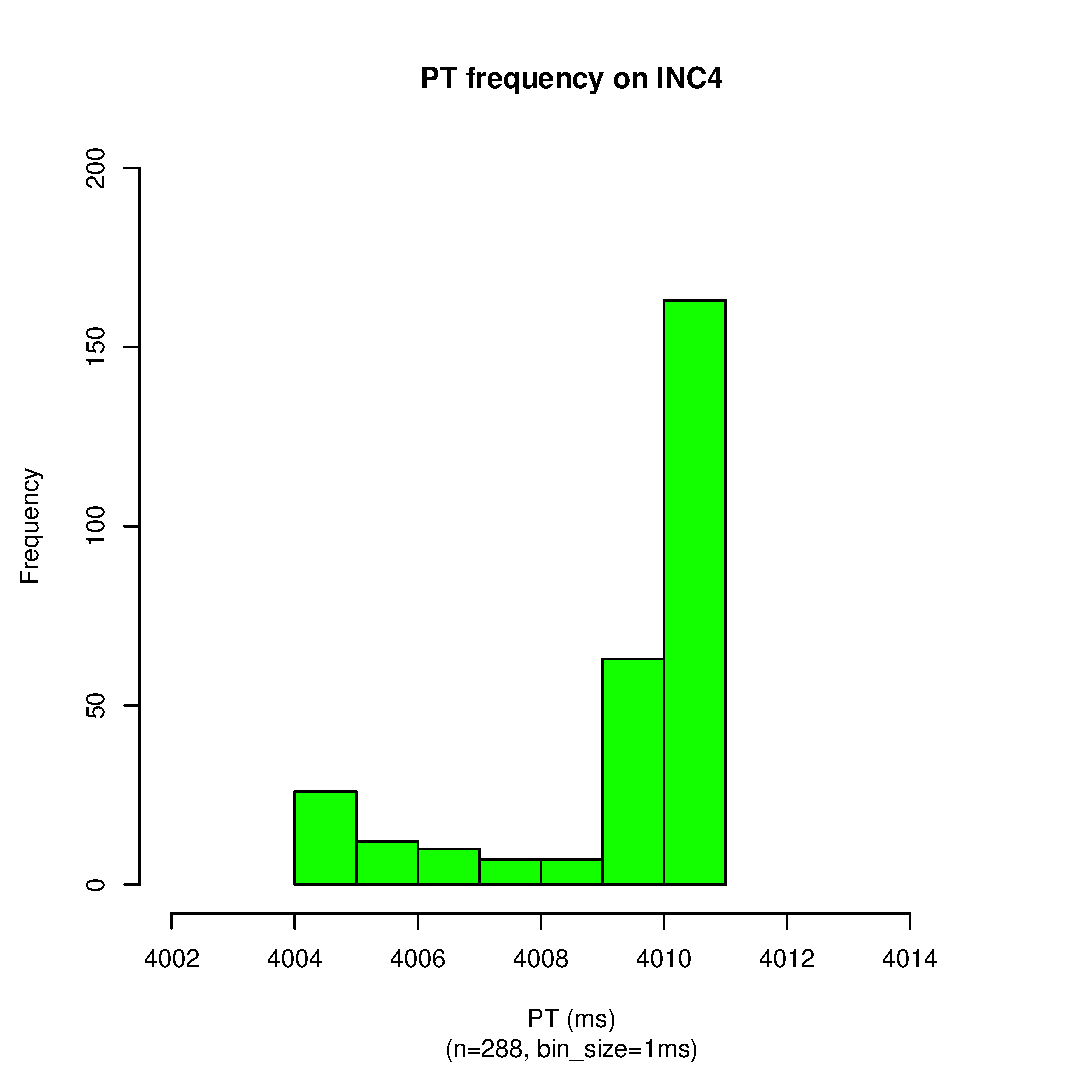
\includegraphics[scale=0.43]{sodb9/4_sec_pt_hist_v5.eps}
		\label{fig:inc4_hist_v5}
	}
	\subfigure[PT frequency on INC8]{
		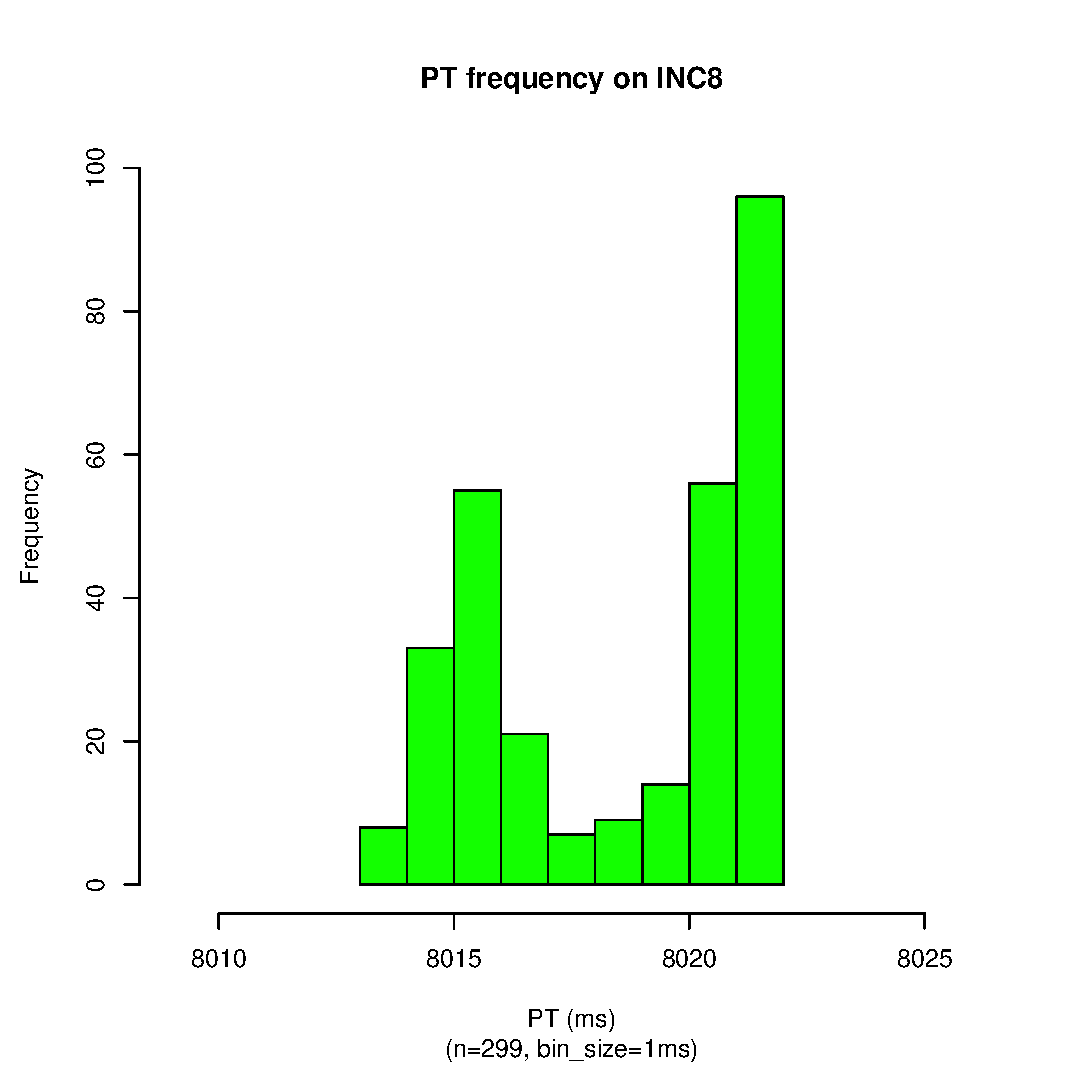
\includegraphics[scale=0.43]{sodb9/8_sec_pt_hist_v5.eps}
		\label{fig:inc8_hist_v5}
	}
	\caption{PT Histograms of INC1 ... INC8~\label{fig:s9_pt_hist1}}
\end{figure}

\begin{figure}[hp!]
	\centering
	\subfigure[PT frequency on INC16]{
		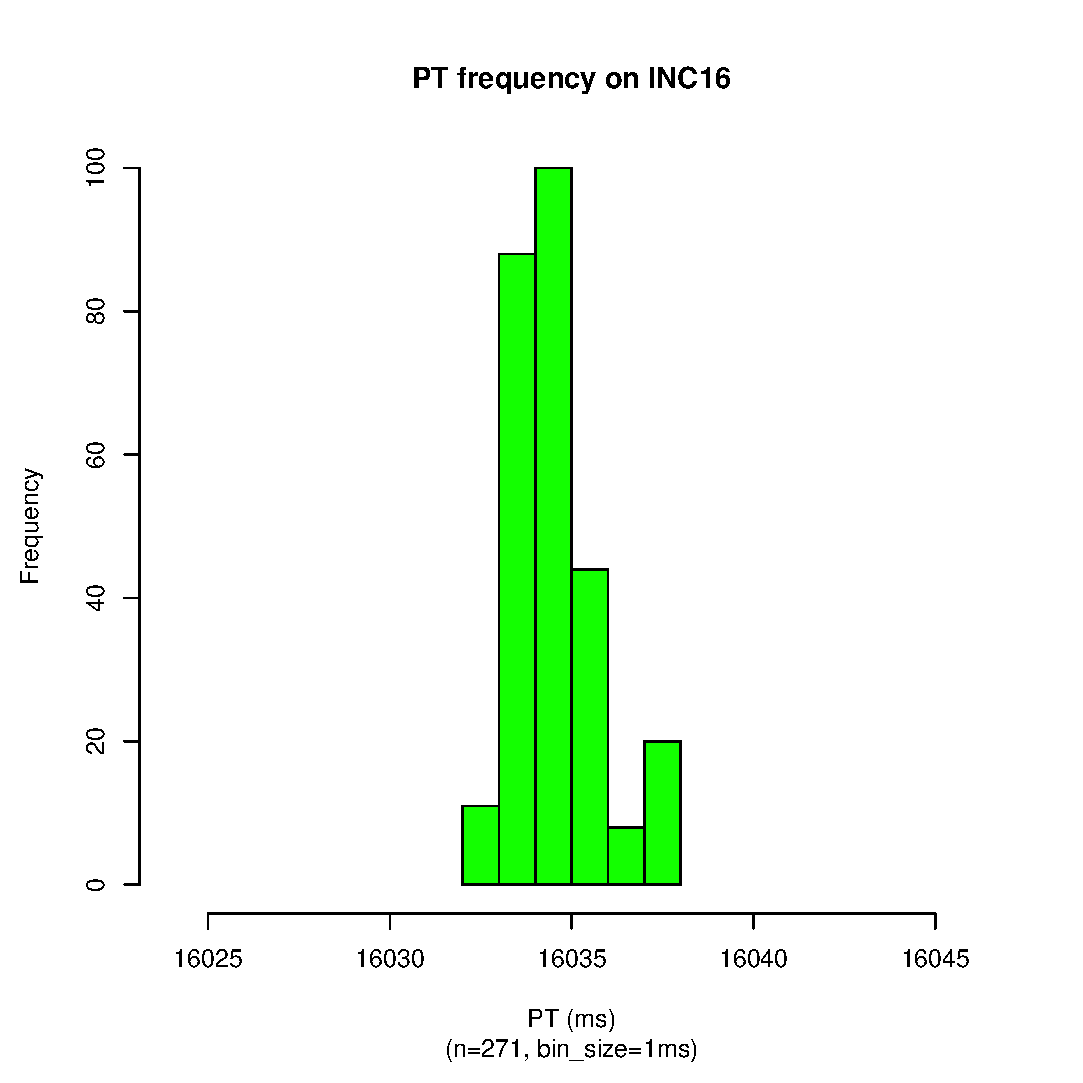
\includegraphics[scale=0.43]{sodb9/16_sec_pt_hist_v5.eps}
		\label{fig:inc16_hist_v5}
	}
	\subfigure[PT frequency on INC32]{
		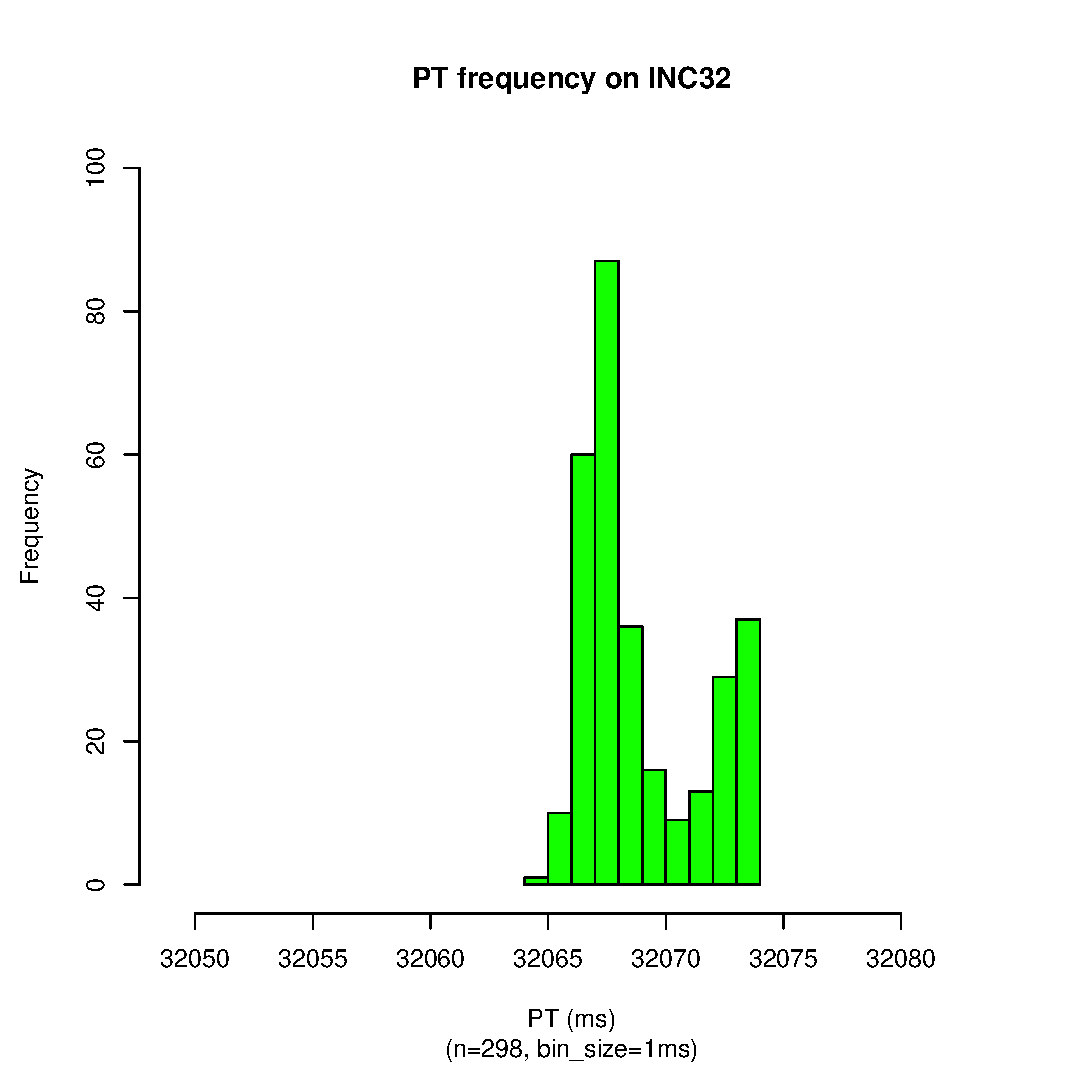
\includegraphics[scale=0.43]{sodb9/32_sec_pt_hist_v5.eps}
		\label{fig:inc32_hist_v5}
	}
	\subfigure[PT frequency on INC64]{
		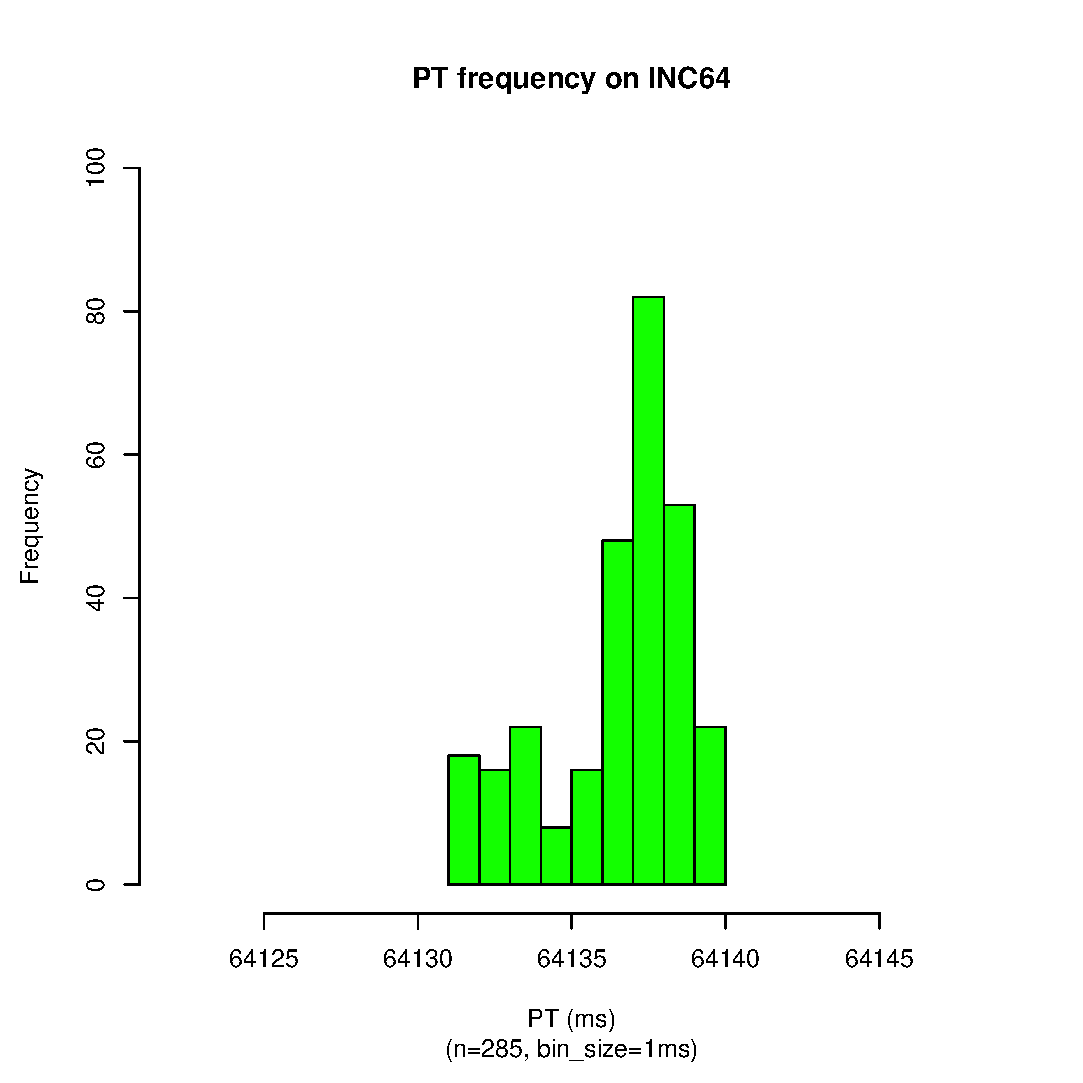
\includegraphics[scale=0.43]{sodb9/64_sec_pt_hist_v5.eps}
		\label{fig:inc64_hist_v5}
	}
	\subfigure[PT frequency on INC128]{
		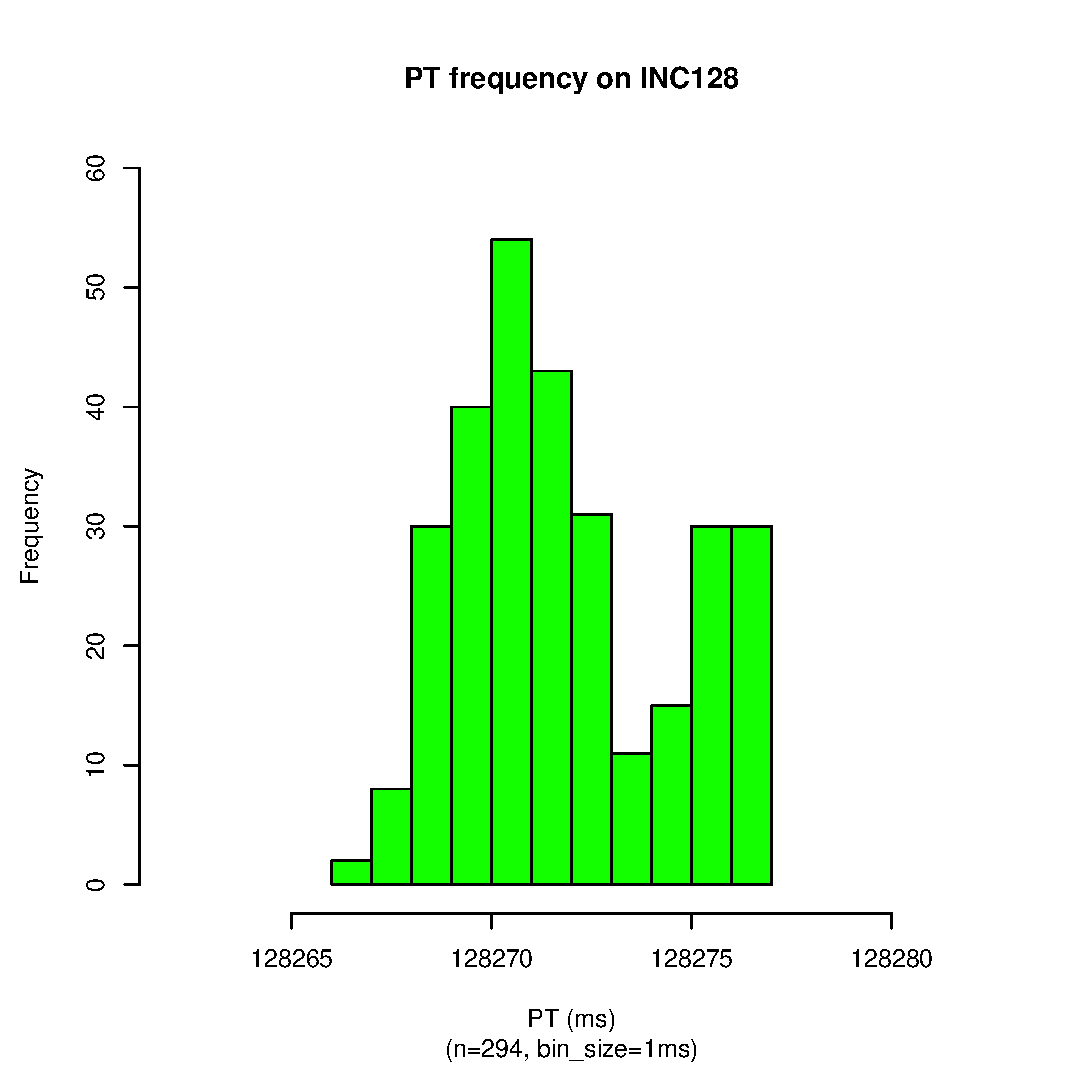
\includegraphics[scale=0.43]{sodb9/128_sec_pt_hist_v5.eps}
		\label{fig:inc128_hist_v5}
	}
	\caption{PT Histograms of INC16 ... INC64~\label{fig:s9_pt_hist2}}
\end{figure}
\newpage

\section{{\tt sodb9}~\label{sec:sodb9_hist}} 
This section exhibits histograms on the EMPv5 data obtained on {\tt sodb9}. 
The detailed description of the base data are from Table~\ref{tab:exp_notes}.

\subsection{ET}

\begin{figure}[hp!]
	\centering
	\subfigure[ET frequency on INC1]{
		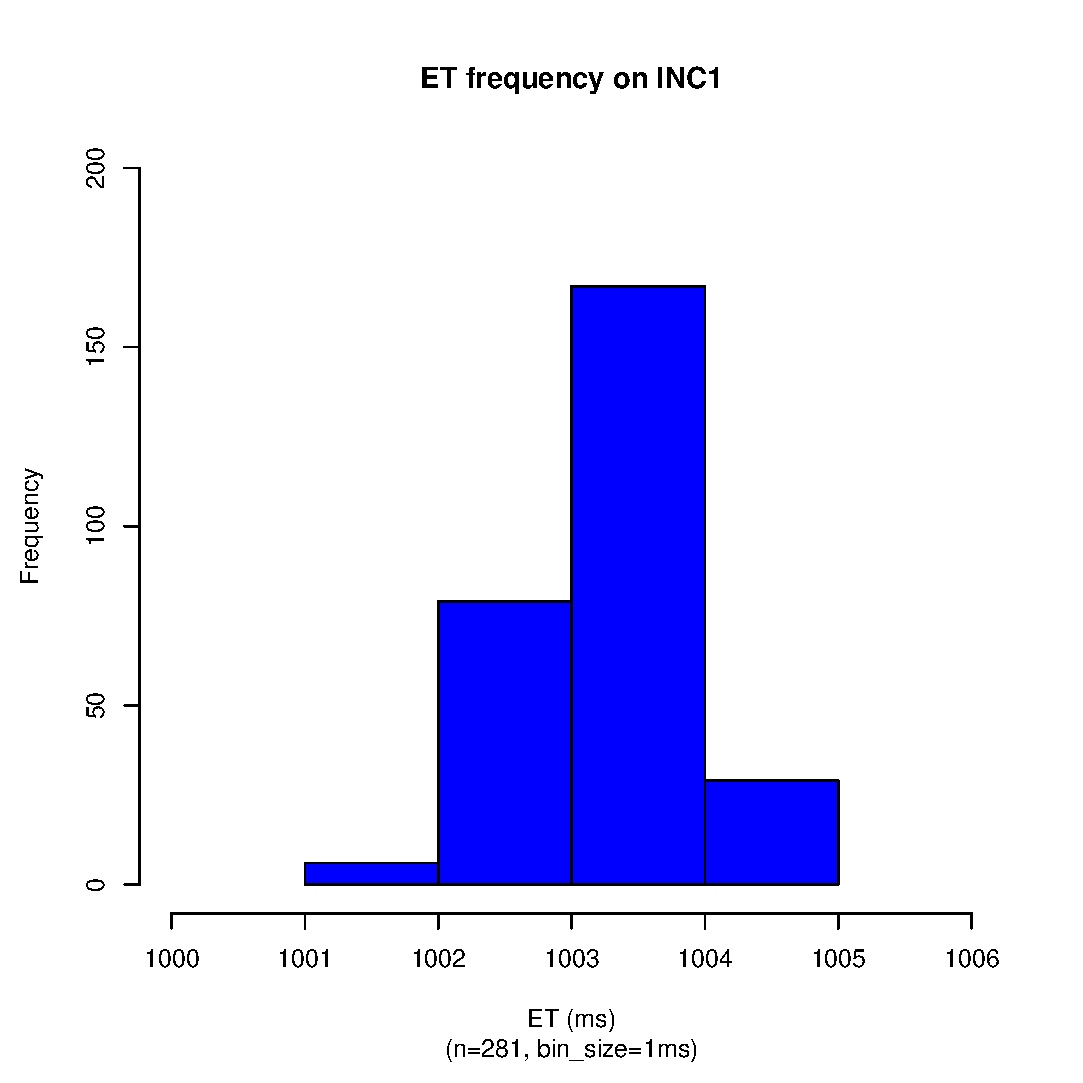
\includegraphics[scale=0.43]{sodb9/1_sec_et_hist_v5.eps}
		\label{fig:inc1_et_hist_v5}
	}
	\subfigure[ET frequency on INC2]{
		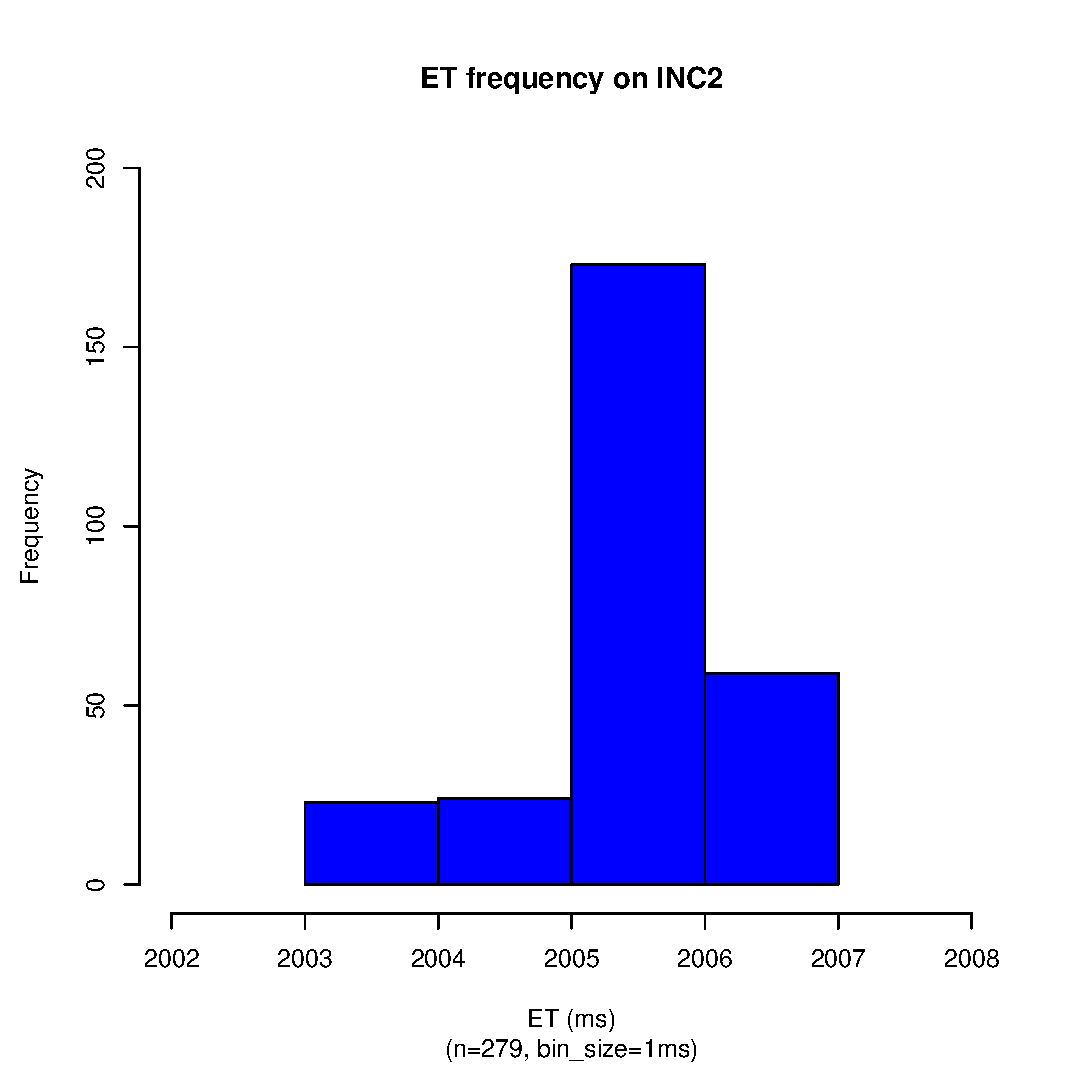
\includegraphics[scale=0.43]{sodb9/2_sec_et_hist_v5.eps}
		\label{fig:inc2_et_hist_v5}
	}
	\subfigure[ET frequency on INC4]{
		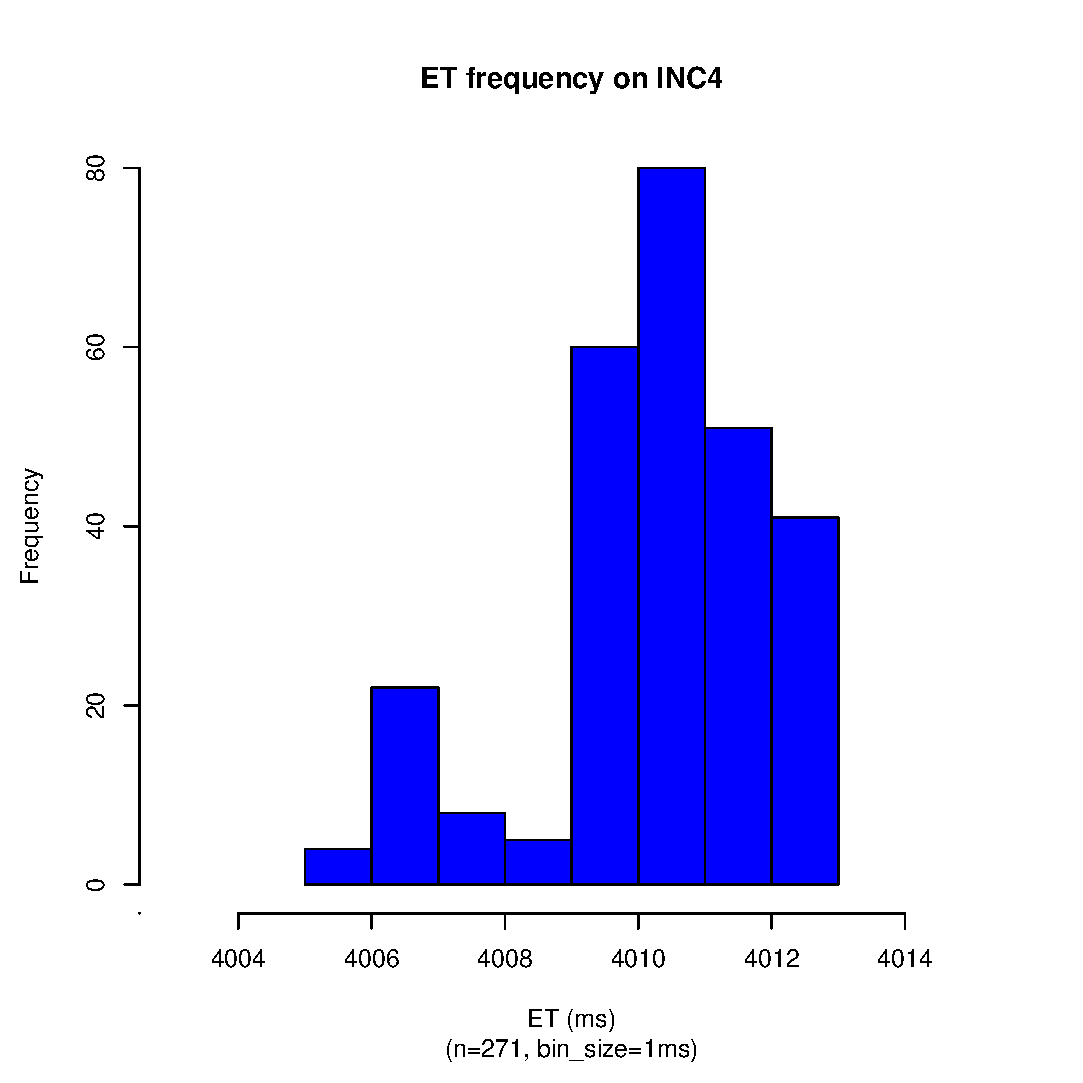
\includegraphics[scale=0.43]{sodb9/4_sec_et_hist_v5.eps}
		\label{fig:inc4_et_hist_v5}
	}
	\subfigure[ET frequency on INC8]{
		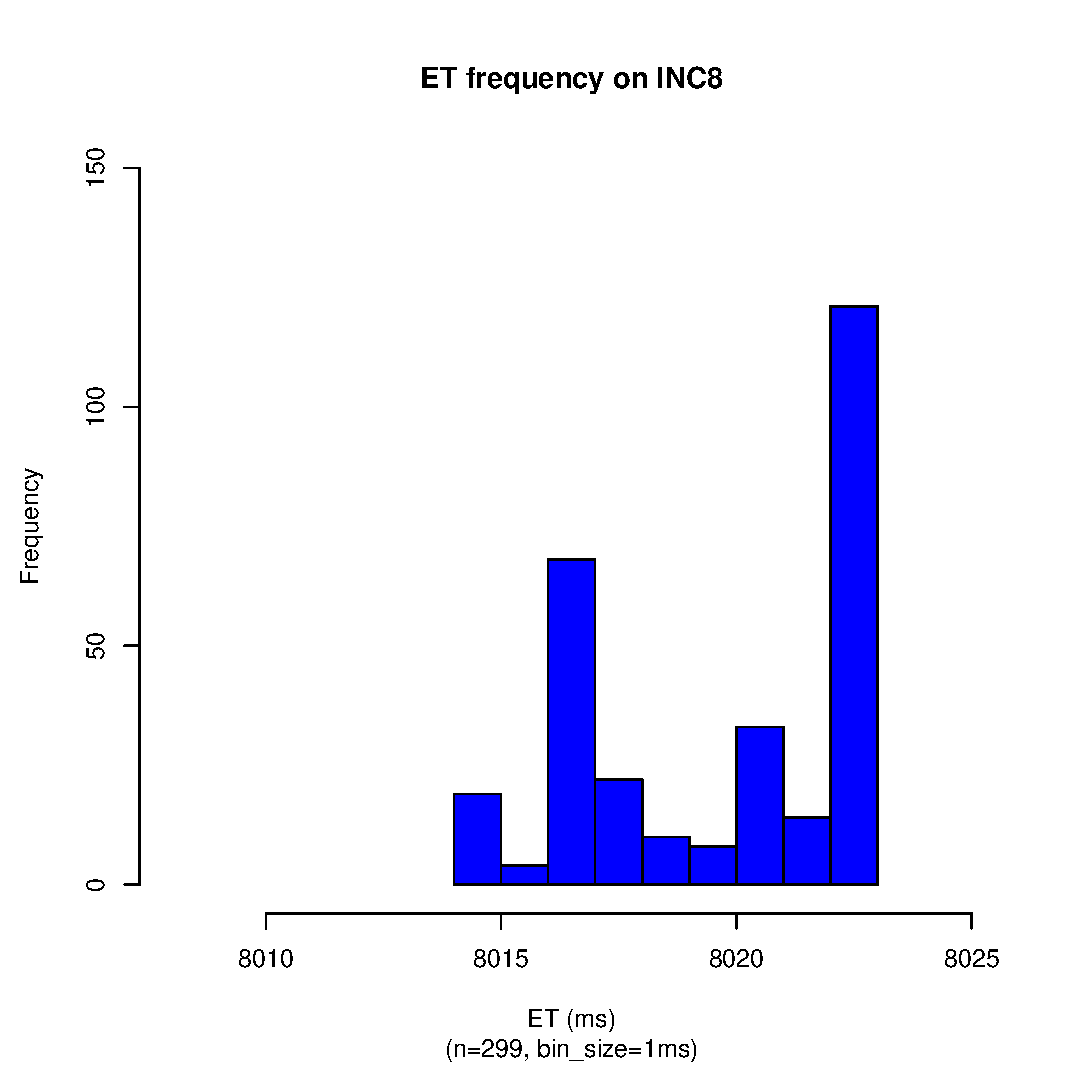
\includegraphics[scale=0.43]{sodb9/8_sec_et_hist_v5.eps}
		\label{fig:inc8_et_hist_v5}
	}
	\caption{ET Histograms of INC1 ... INC8~\label{fig:s9_et_hist1}}
\end{figure}

\begin{figure}[hp!]
	\centering
	\subfigure[ET frequency on INC16]{
		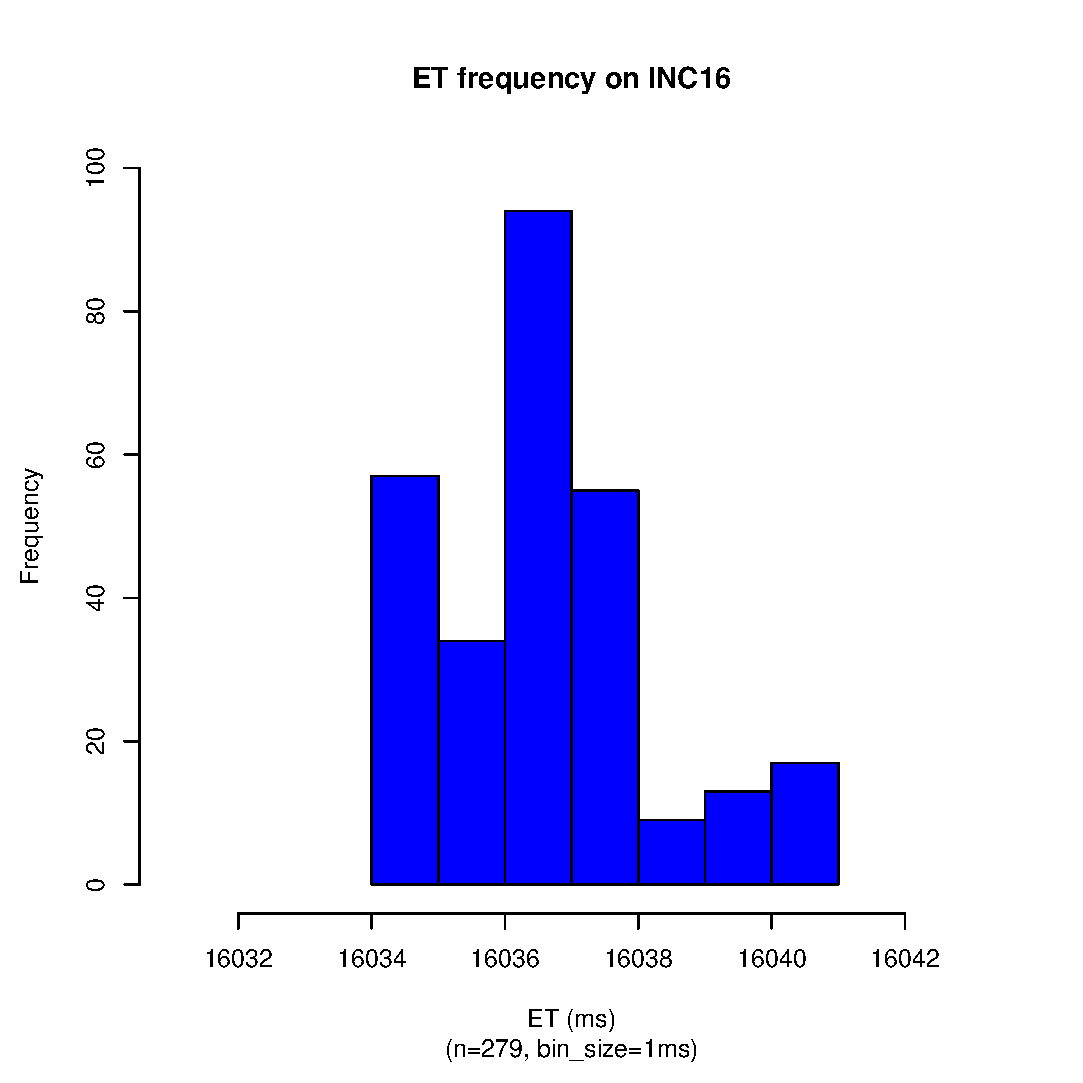
\includegraphics[scale=0.43]{sodb9/16_sec_et_hist_v5.eps}
		\label{fig:inc16_et_hist_v5}
	}
	\subfigure[ET frequency on INC32]{
		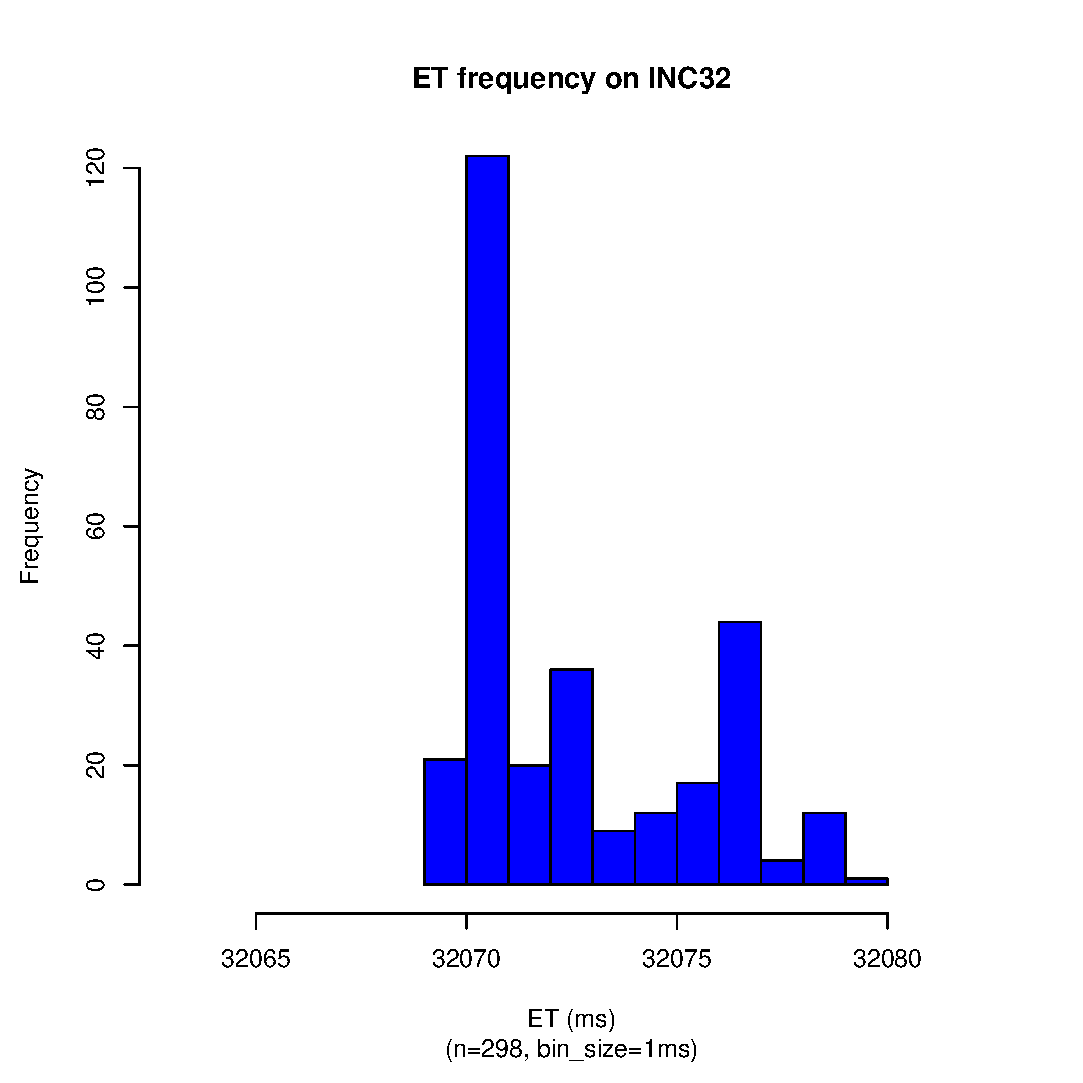
\includegraphics[scale=0.43]{sodb9/32_sec_et_hist_v5.eps}
		\label{fig:inc32_et_hist_v5}
	}
	\subfigure[ET frequency on INC64]{
		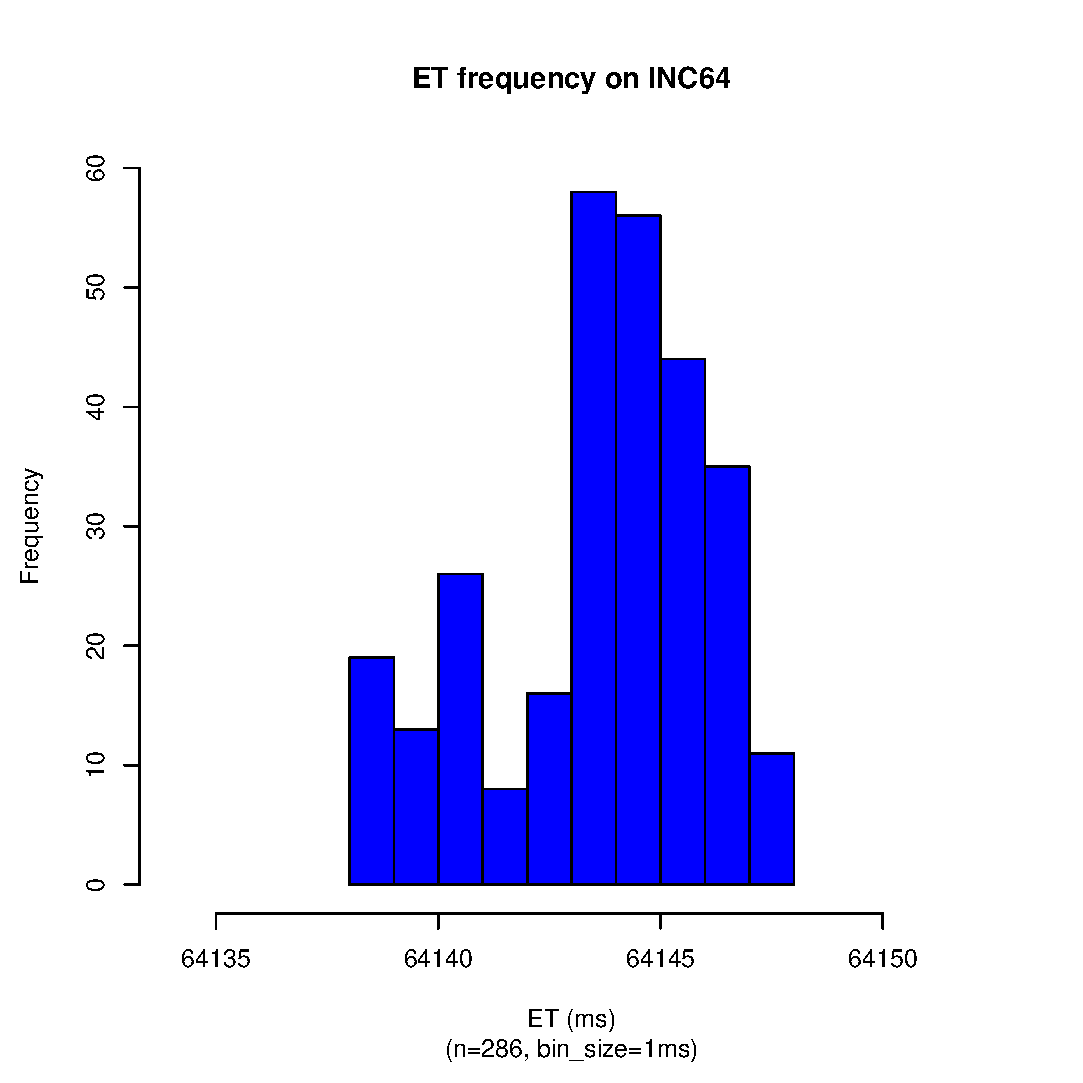
\includegraphics[scale=0.43]{sodb9/64_sec_et_hist_v5.eps}
		\label{fig:inc64_et_hist_v5}
	}
	\subfigure[ET frequency on INC128]{
		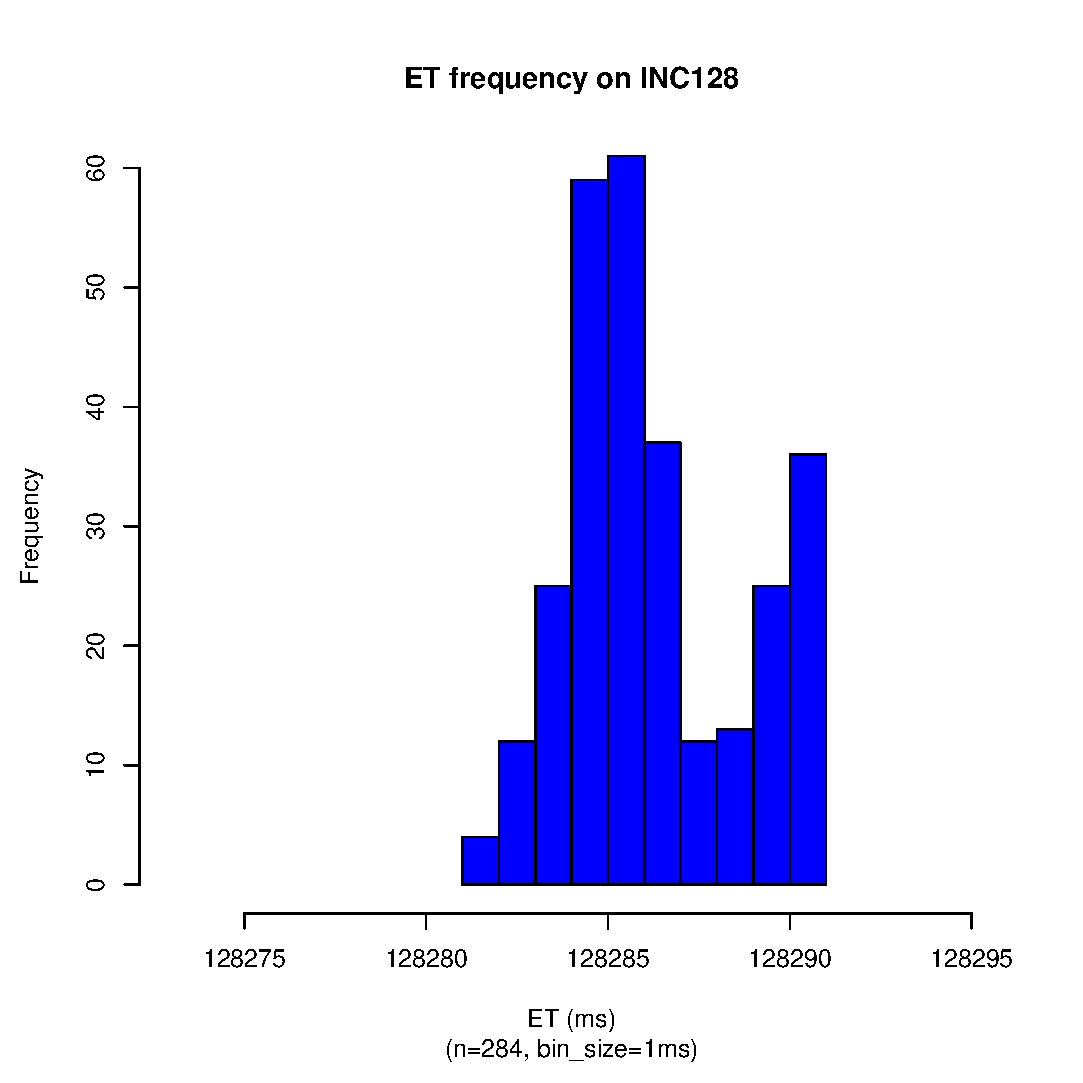
\includegraphics[scale=0.43]{sodb9/128_sec_et_hist_v5.eps}
		\label{fig:inc128_et_hist_v5}
	}
	\caption{ET Histograms of INC16 ... INC128~\label{fig:s9_et_hist2}}
\end{figure}

\newpage

\subsection{PT}

\begin{figure}[hp!]
	\centering
	\subfigure[PT frequency on INC1]{
		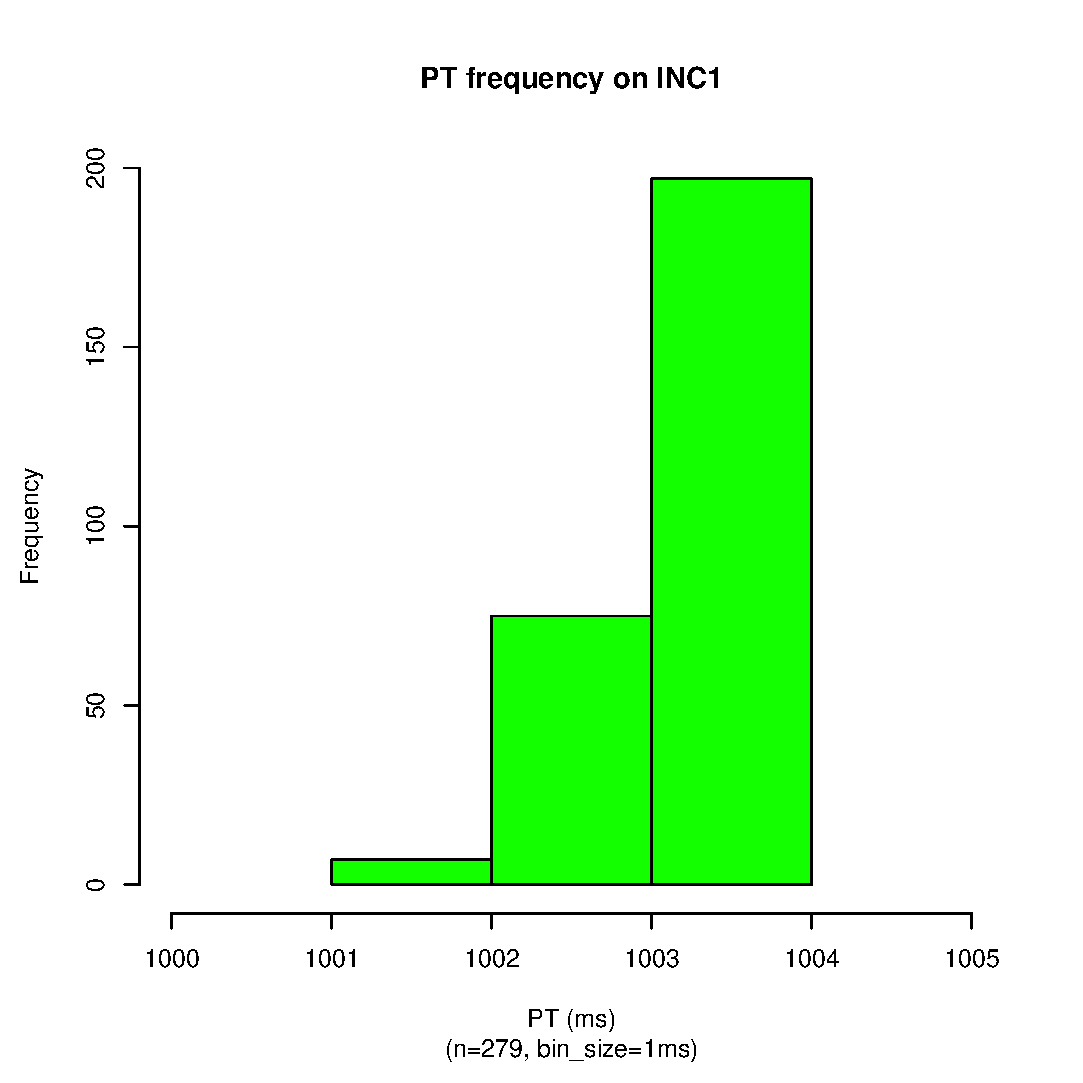
\includegraphics[scale=0.43]{sodb9/1_sec_pt_hist_v5.eps}
		\label{fig:inc1_hist_v5}
	}
	\subfigure[PT frequency on INC2]{
		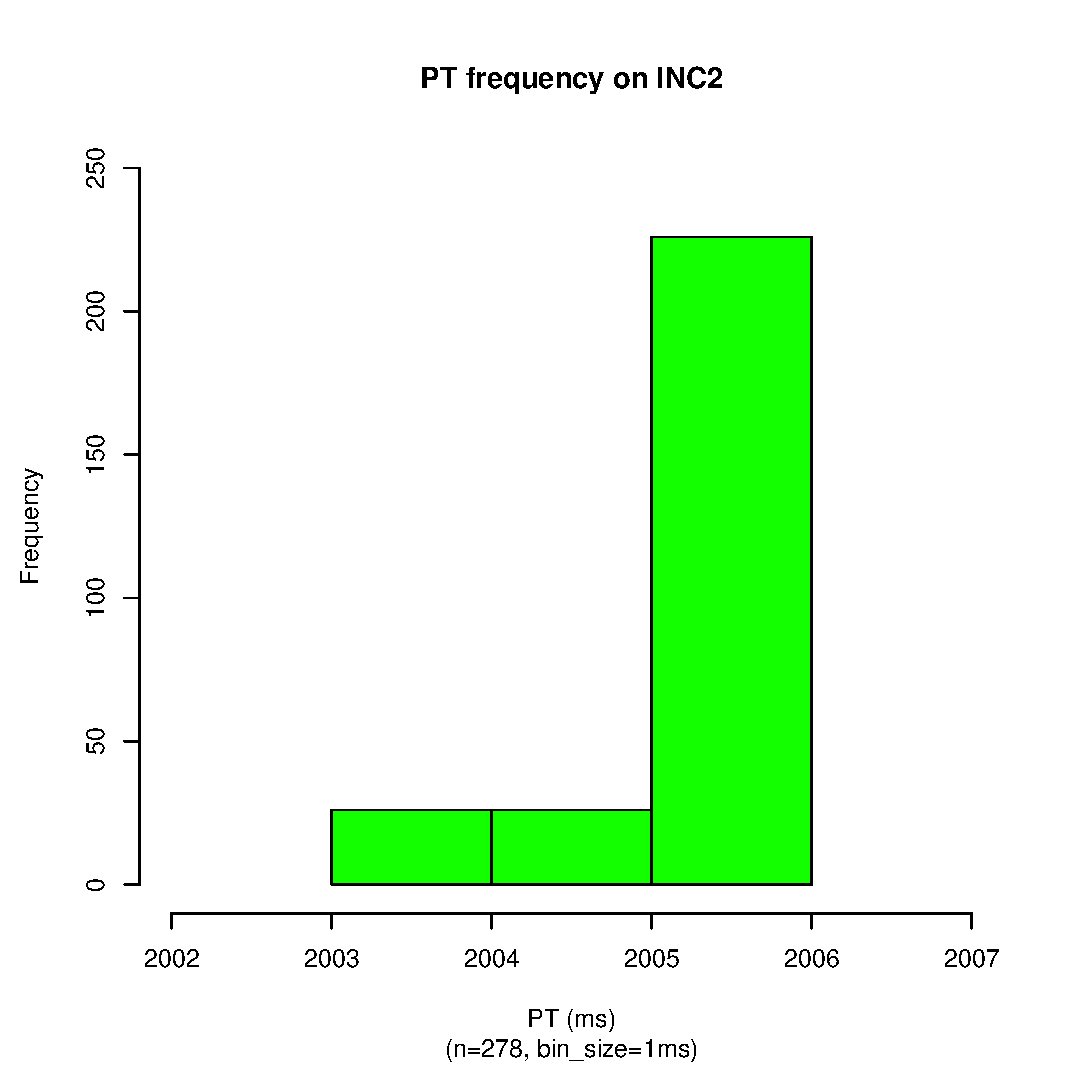
\includegraphics[scale=0.43]{sodb9/2_sec_pt_hist_v5.eps}
		\label{fig:inc2_hist_v5}
	}
	\subfigure[PT frequency on INC4]{
		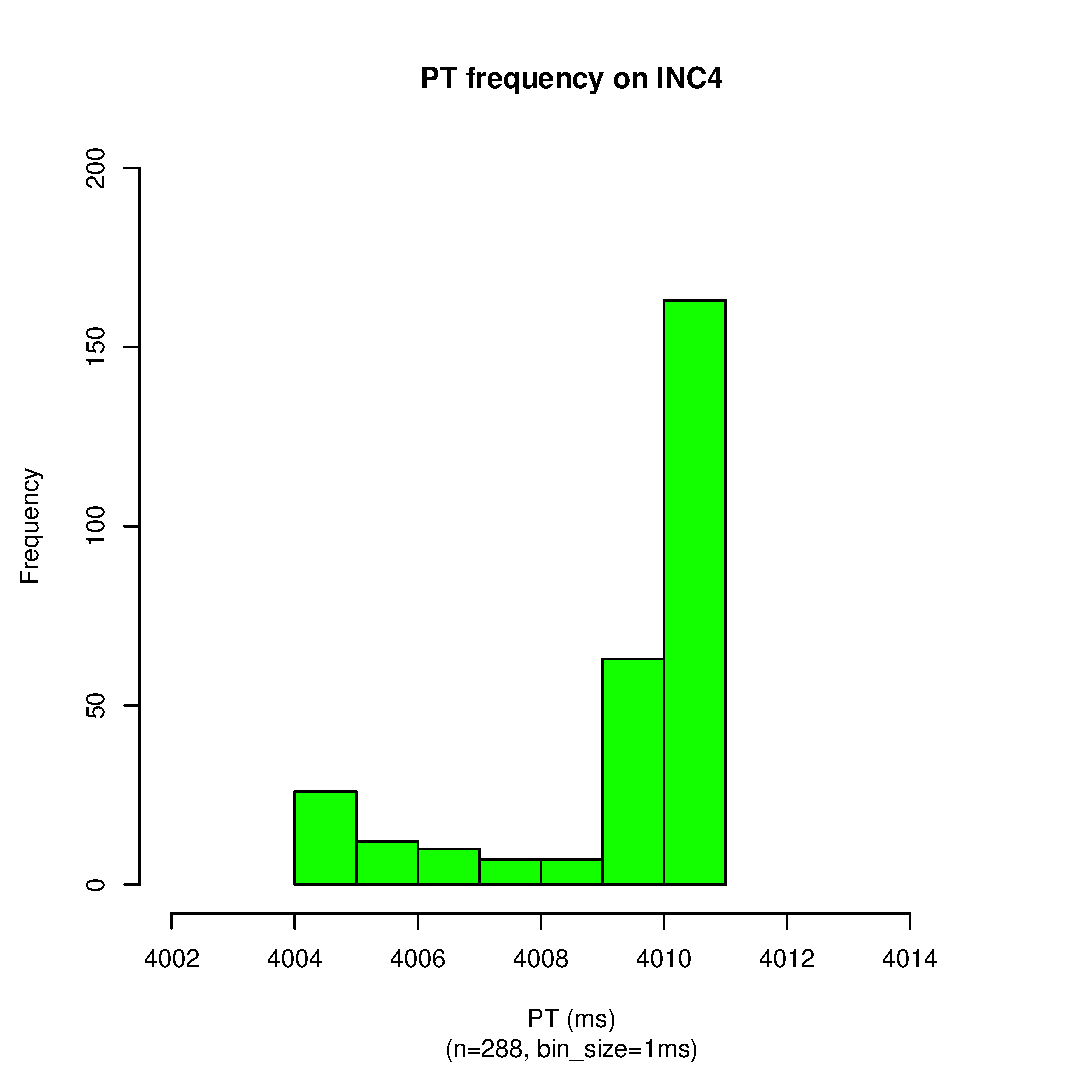
\includegraphics[scale=0.43]{sodb9/4_sec_pt_hist_v5.eps}
		\label{fig:inc4_hist_v5}
	}
	\subfigure[PT frequency on INC8]{
		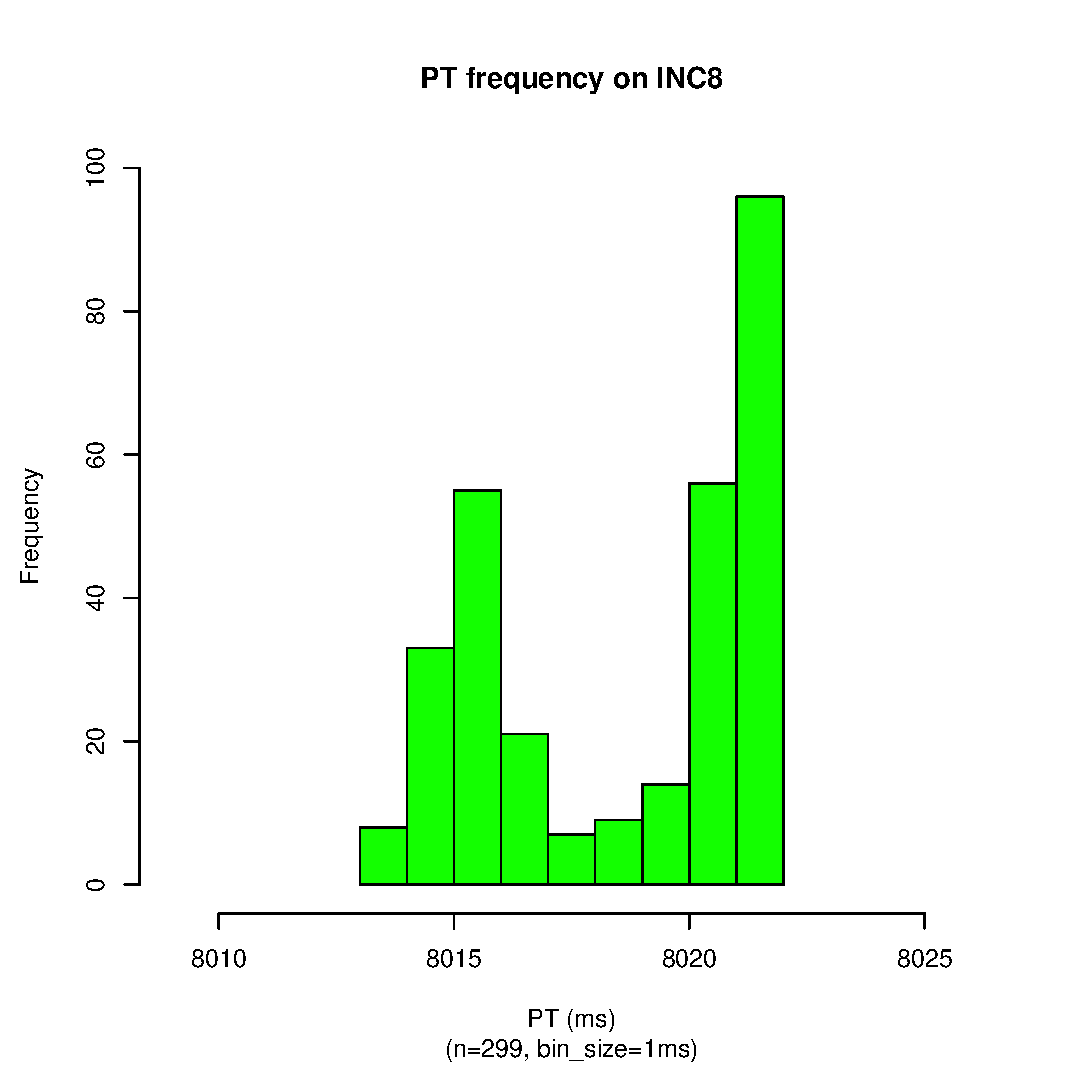
\includegraphics[scale=0.43]{sodb9/8_sec_pt_hist_v5.eps}
		\label{fig:inc8_hist_v5}
	}
	\caption{PT Histograms of INC1 ... INC8~\label{fig:s9_pt_hist1}}
\end{figure}

\begin{figure}[hp!]
	\centering
	\subfigure[PT frequency on INC16]{
		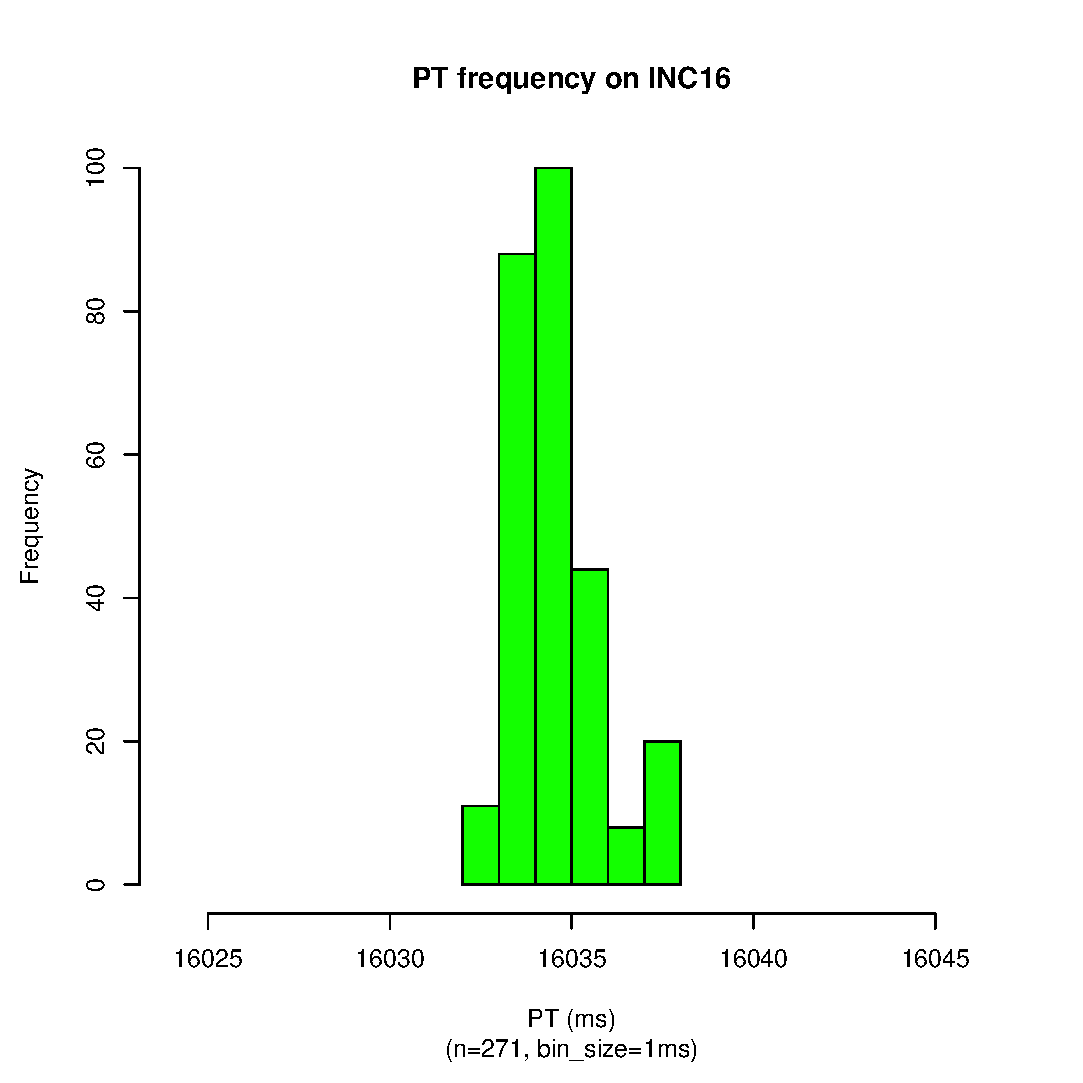
\includegraphics[scale=0.43]{sodb9/16_sec_pt_hist_v5.eps}
		\label{fig:inc16_hist_v5}
	}
	\subfigure[PT frequency on INC32]{
		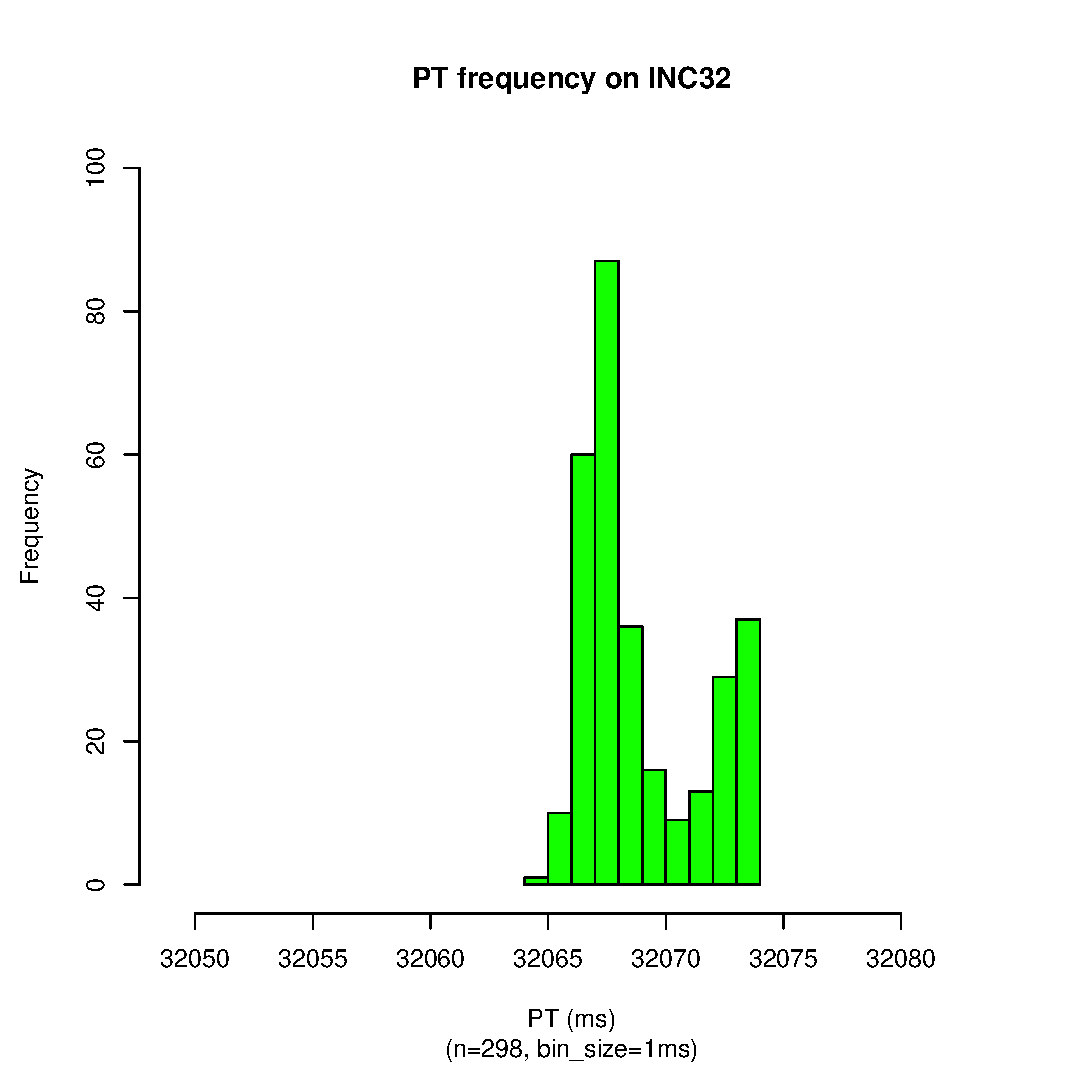
\includegraphics[scale=0.43]{sodb9/32_sec_pt_hist_v5.eps}
		\label{fig:inc32_hist_v5}
	}
	\subfigure[PT frequency on INC64]{
		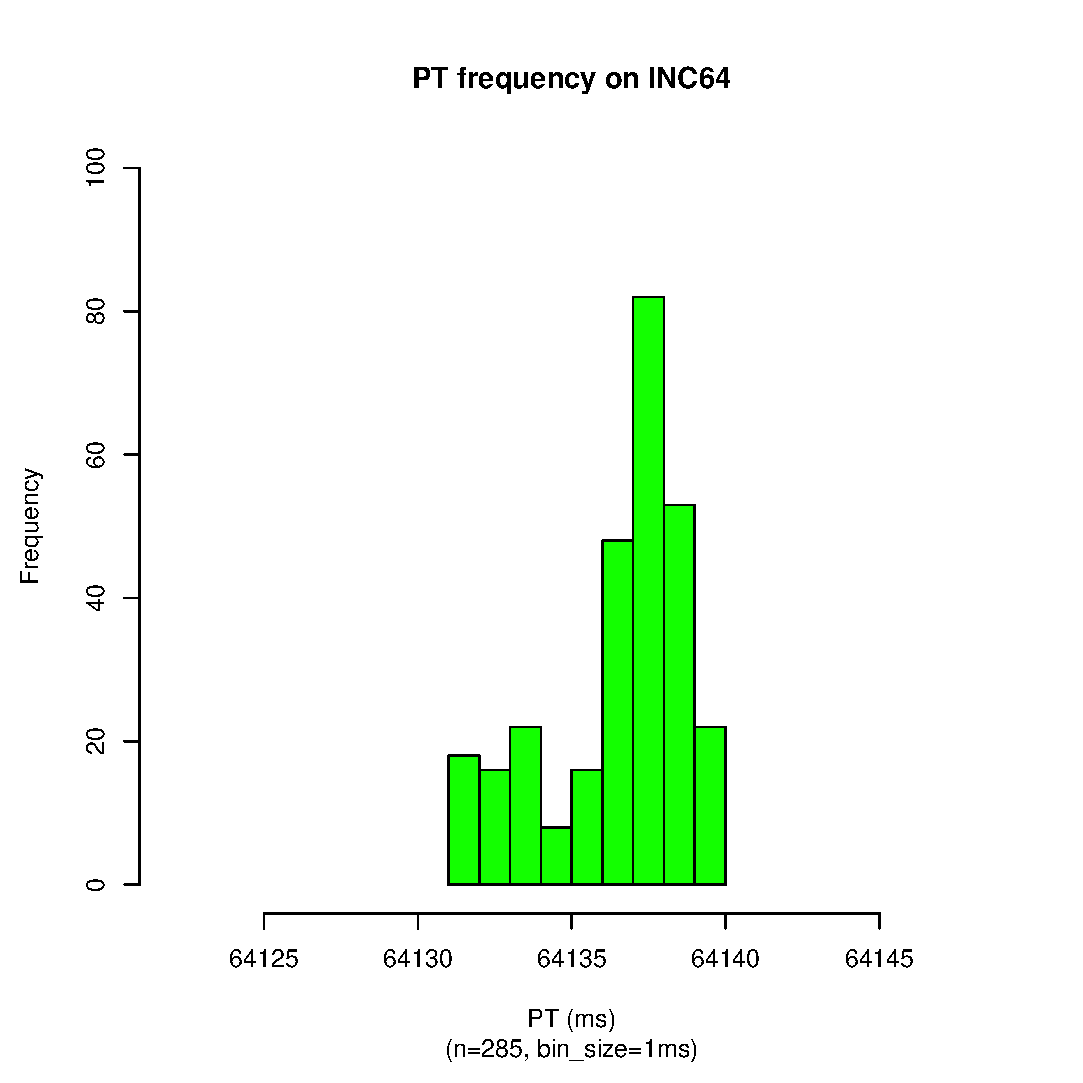
\includegraphics[scale=0.43]{sodb9/64_sec_pt_hist_v5.eps}
		\label{fig:inc64_hist_v5}
	}
	\subfigure[PT frequency on INC128]{
		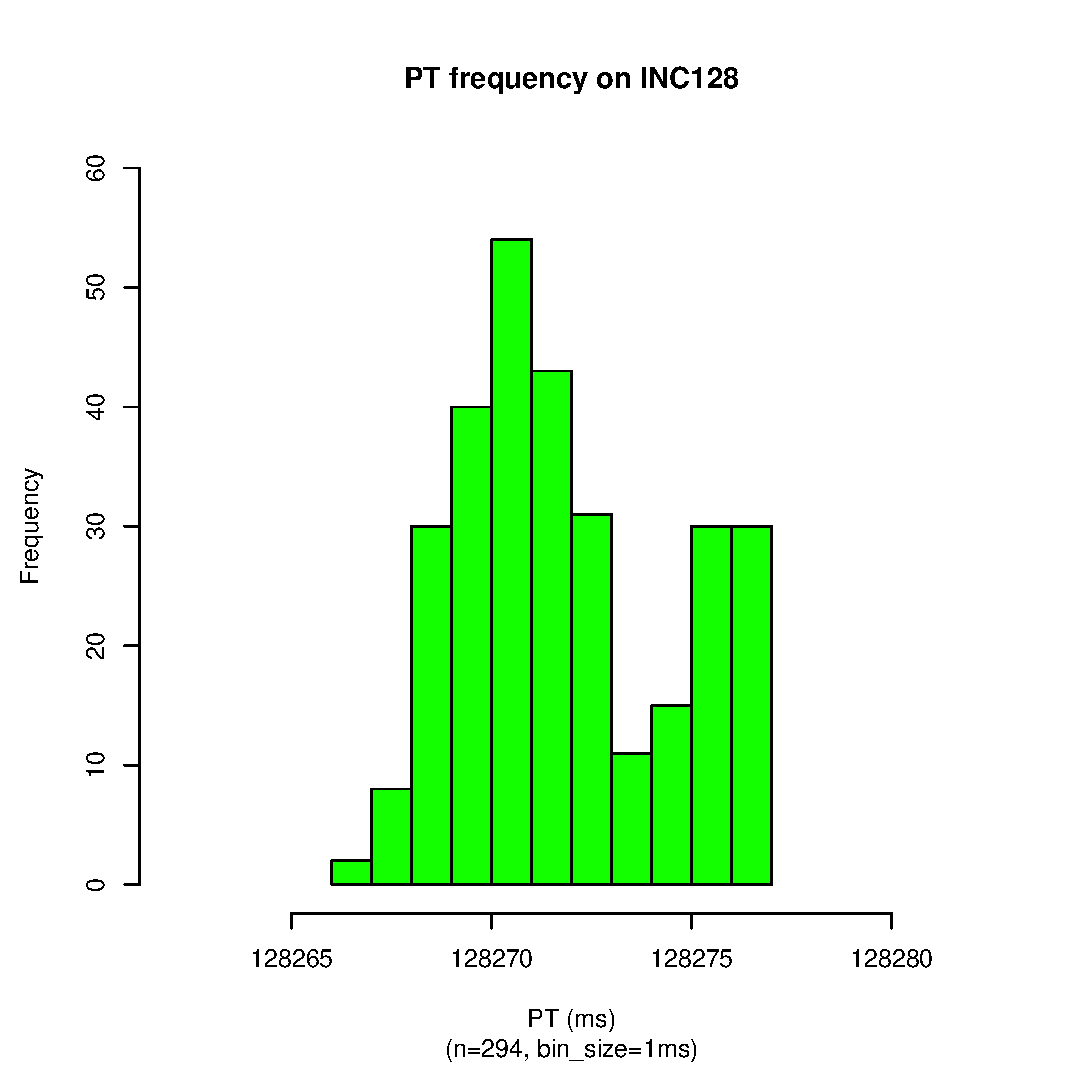
\includegraphics[scale=0.43]{sodb9/128_sec_pt_hist_v5.eps}
		\label{fig:inc128_hist_v5}
	}
	\caption{PT Histograms of INC16 ... INC64~\label{fig:s9_pt_hist2}}
\end{figure}
\newpage

\section{{\tt sodb9}~\label{sec:sodb9_hist}} 
This section exhibits histograms on the EMPv5 data obtained on {\tt sodb9}. 
The detailed description of the base data are from Table~\ref{tab:exp_notes}.

\subsection{ET}

\begin{figure}[hp!]
	\centering
	\subfigure[ET frequency on INC1]{
		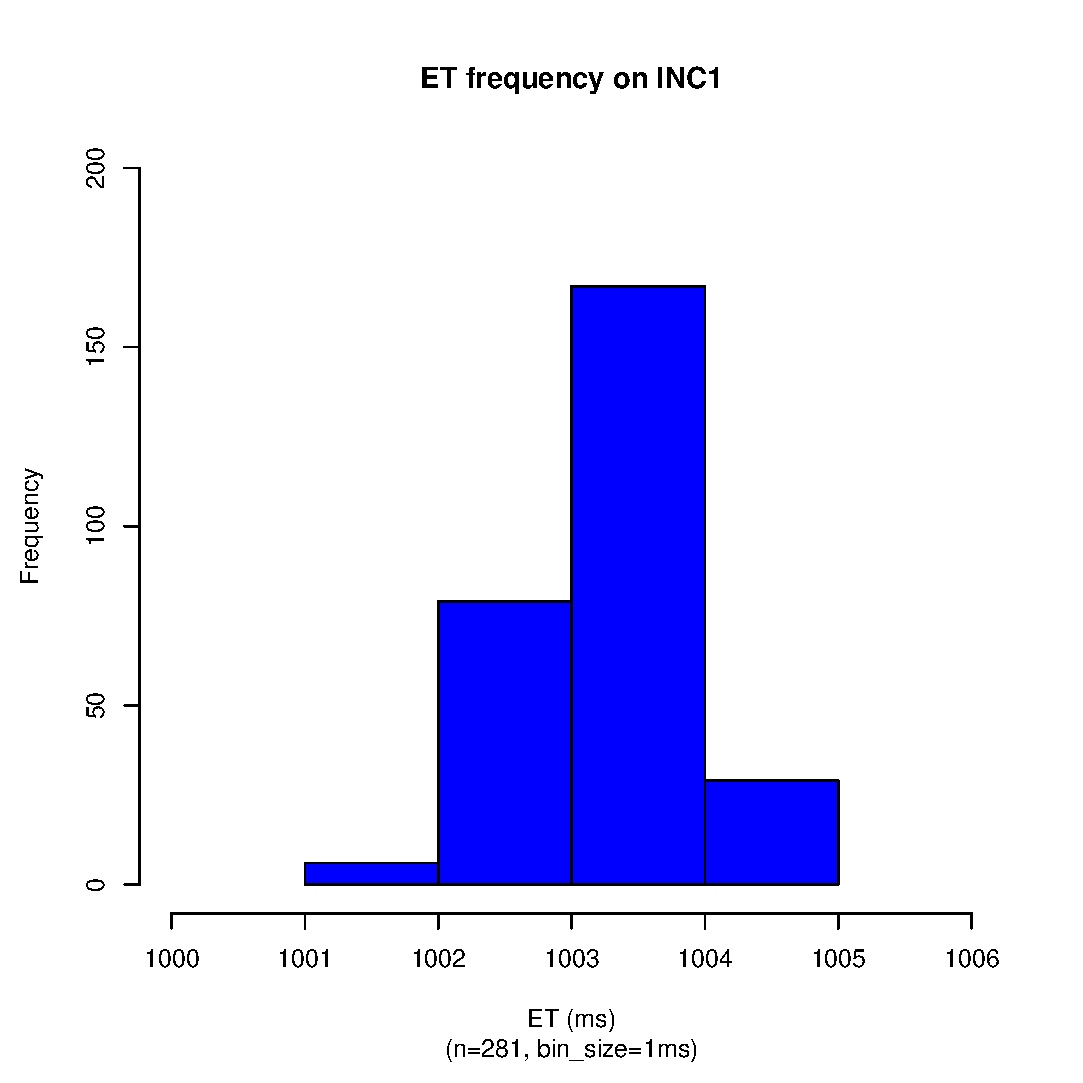
\includegraphics[scale=0.43]{sodb9/1_sec_et_hist_v5.eps}
		\label{fig:inc1_et_hist_v5}
	}
	\subfigure[ET frequency on INC2]{
		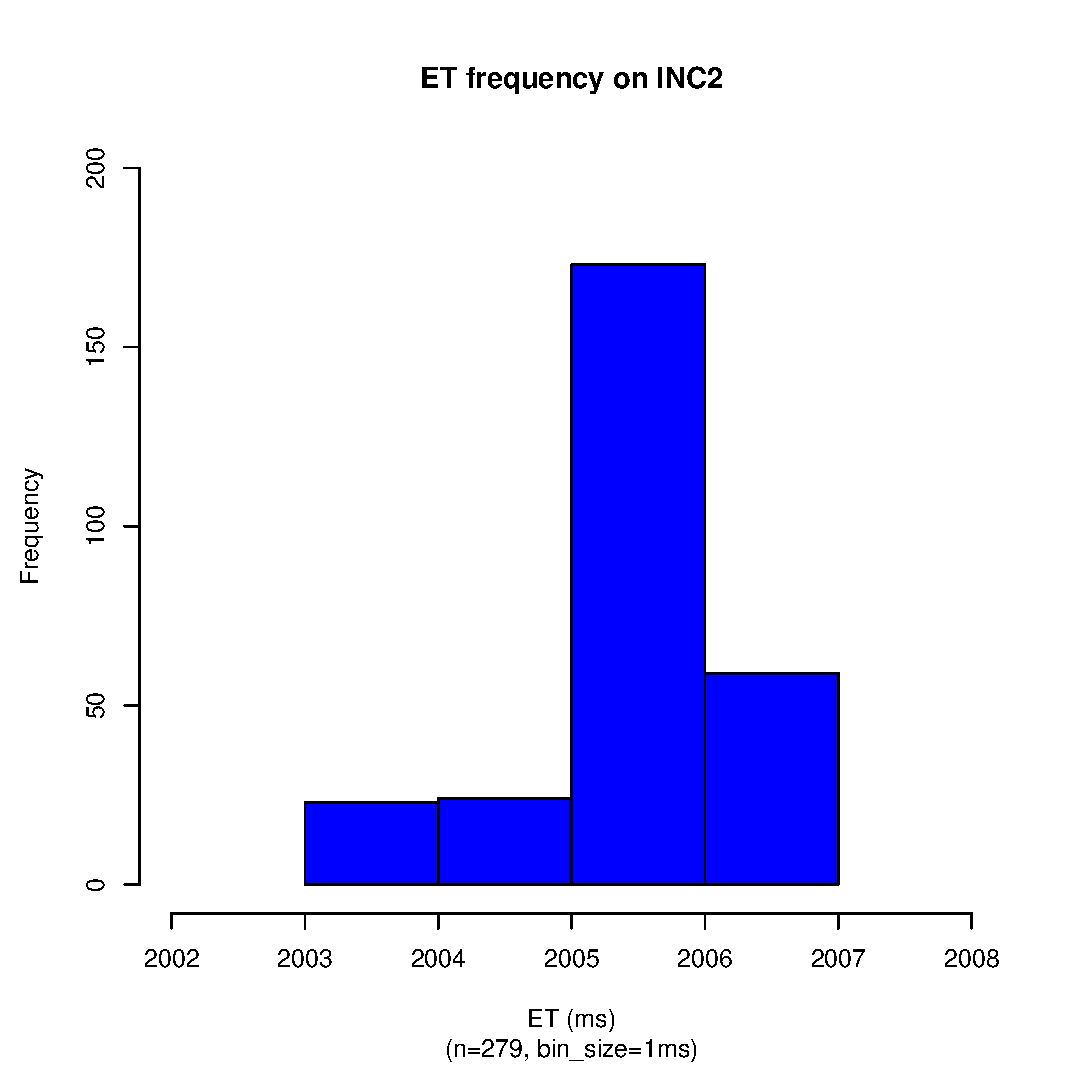
\includegraphics[scale=0.43]{sodb9/2_sec_et_hist_v5.eps}
		\label{fig:inc2_et_hist_v5}
	}
	\subfigure[ET frequency on INC4]{
		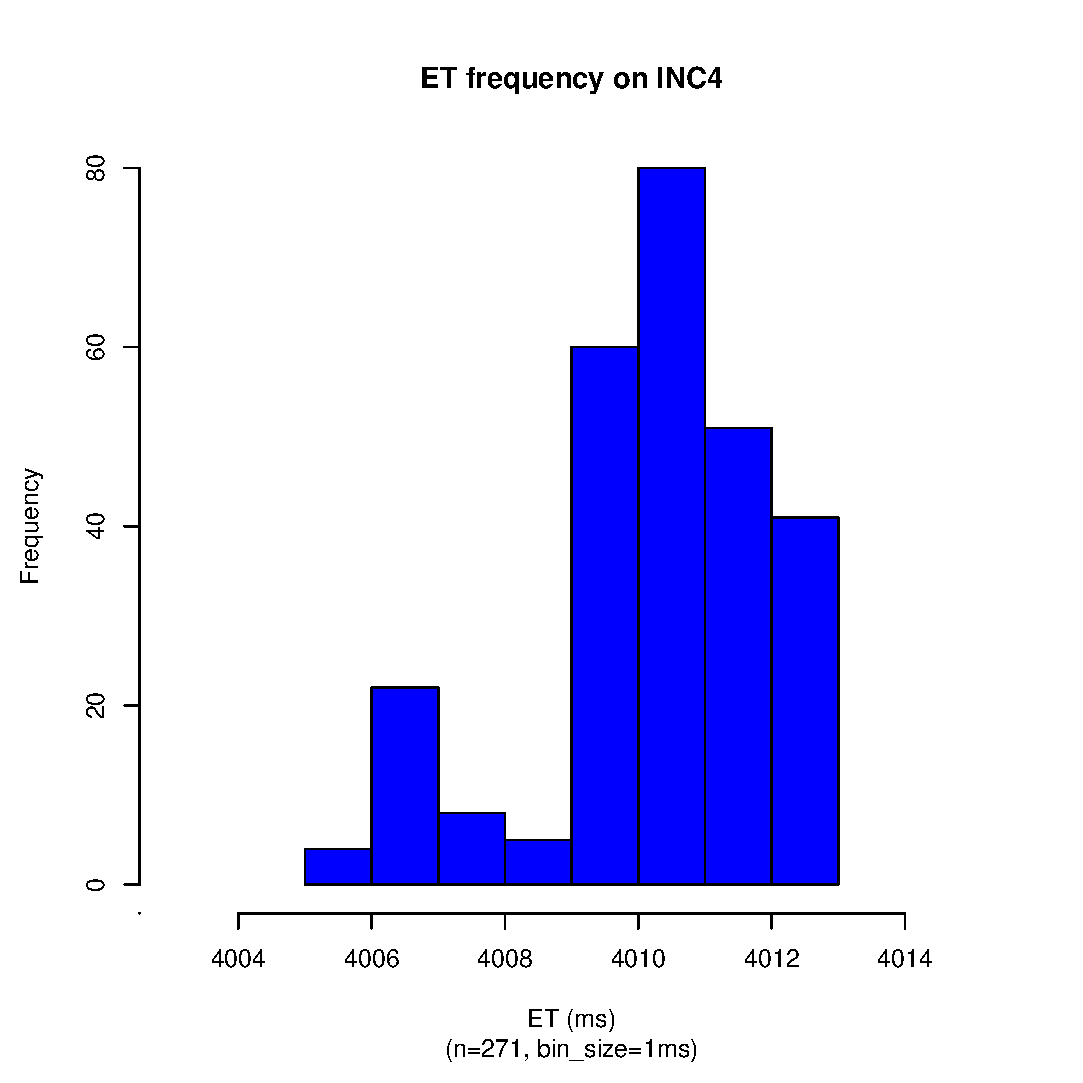
\includegraphics[scale=0.43]{sodb9/4_sec_et_hist_v5.eps}
		\label{fig:inc4_et_hist_v5}
	}
	\subfigure[ET frequency on INC8]{
		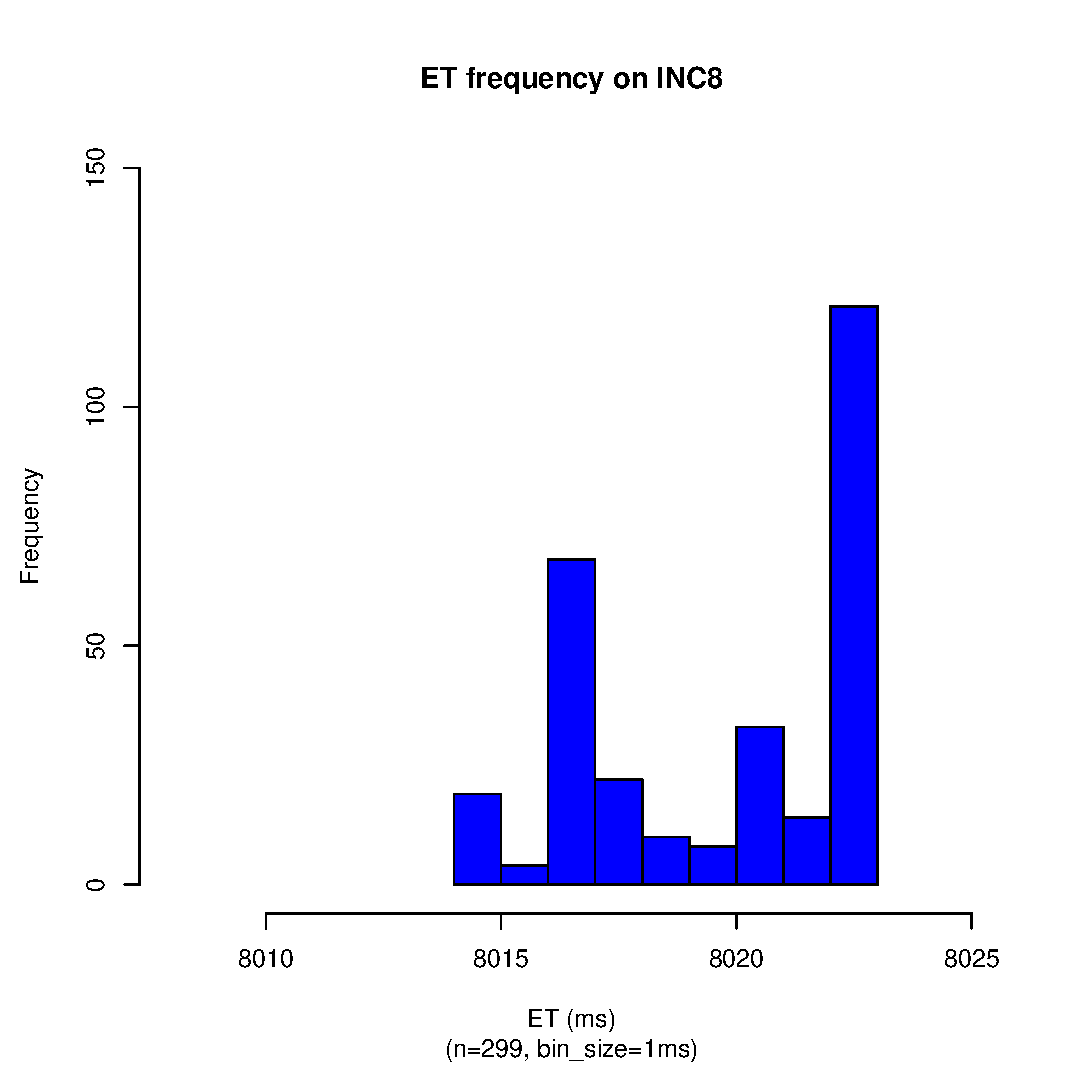
\includegraphics[scale=0.43]{sodb9/8_sec_et_hist_v5.eps}
		\label{fig:inc8_et_hist_v5}
	}
	\caption{ET Histograms of INC1 ... INC8~\label{fig:s9_et_hist1}}
\end{figure}

\begin{figure}[hp!]
	\centering
	\subfigure[ET frequency on INC16]{
		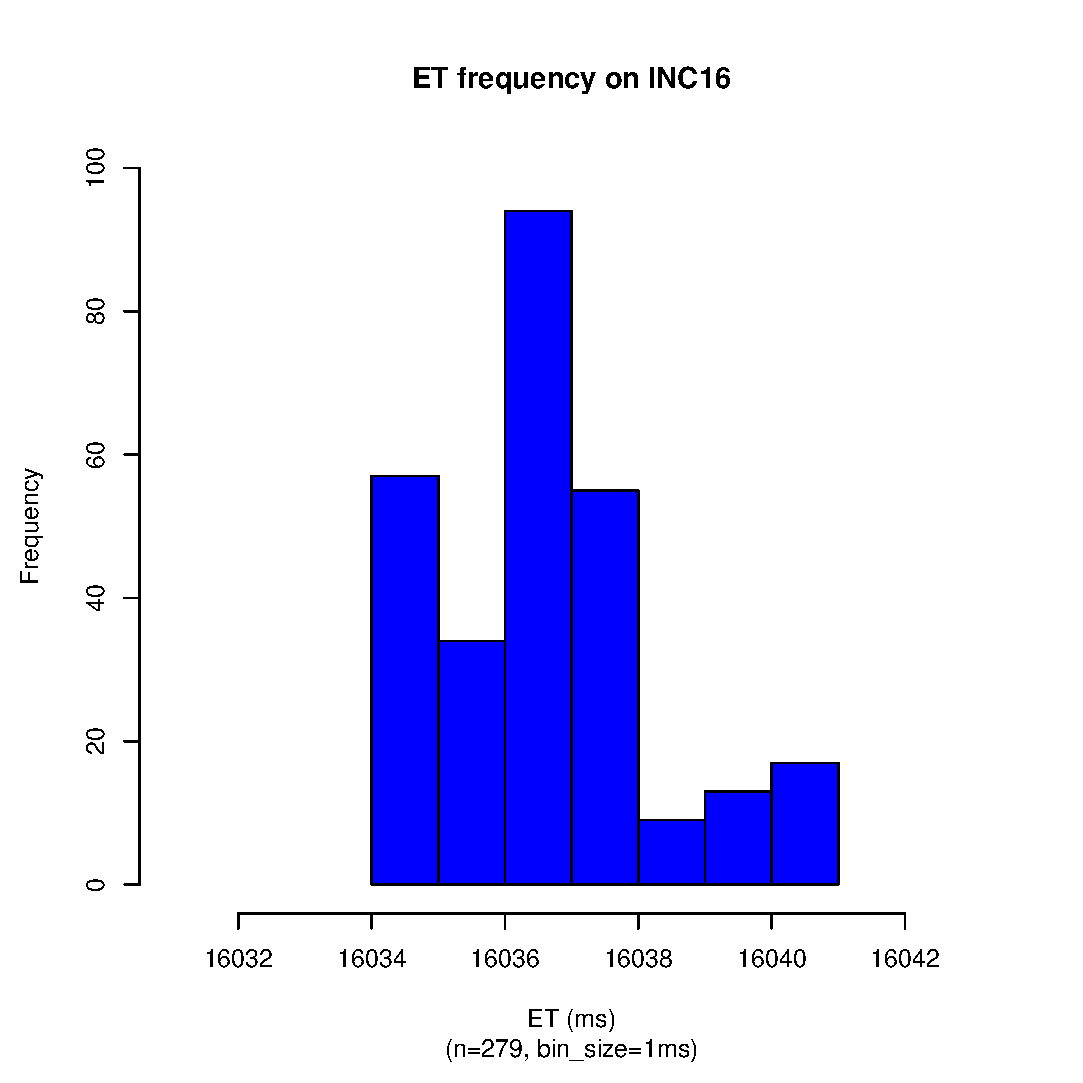
\includegraphics[scale=0.43]{sodb9/16_sec_et_hist_v5.eps}
		\label{fig:inc16_et_hist_v5}
	}
	\subfigure[ET frequency on INC32]{
		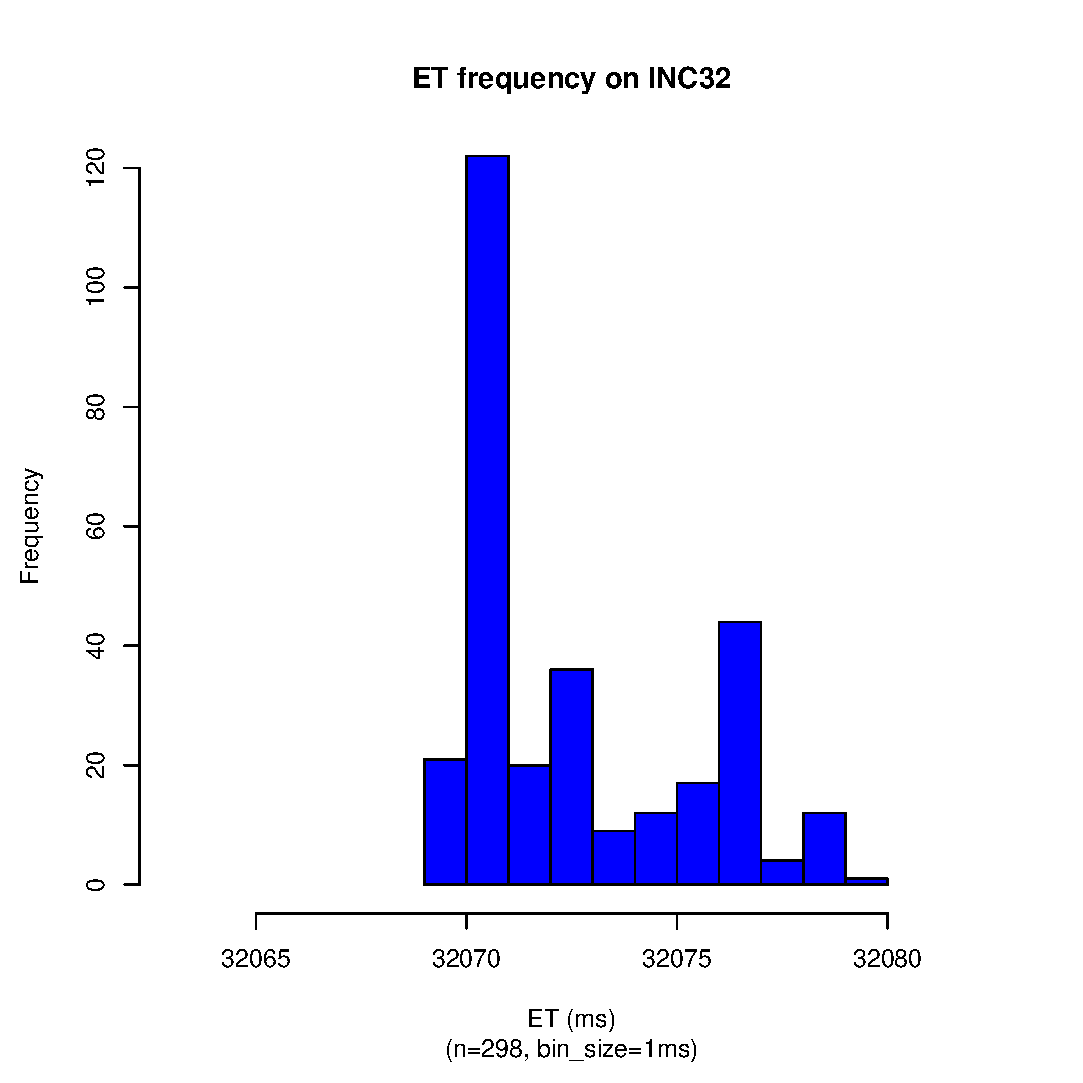
\includegraphics[scale=0.43]{sodb9/32_sec_et_hist_v5.eps}
		\label{fig:inc32_et_hist_v5}
	}
	\subfigure[ET frequency on INC64]{
		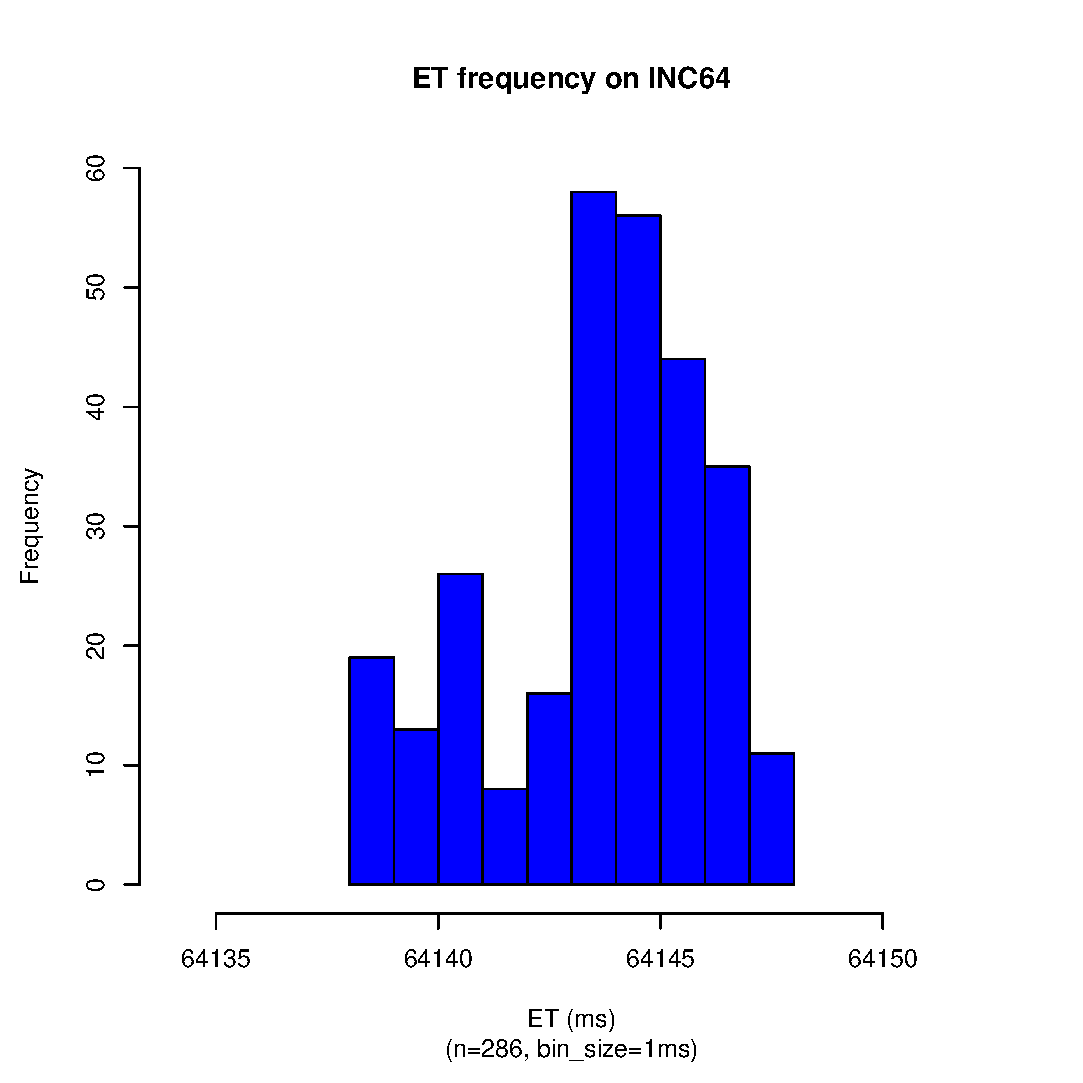
\includegraphics[scale=0.43]{sodb9/64_sec_et_hist_v5.eps}
		\label{fig:inc64_et_hist_v5}
	}
	\subfigure[ET frequency on INC128]{
		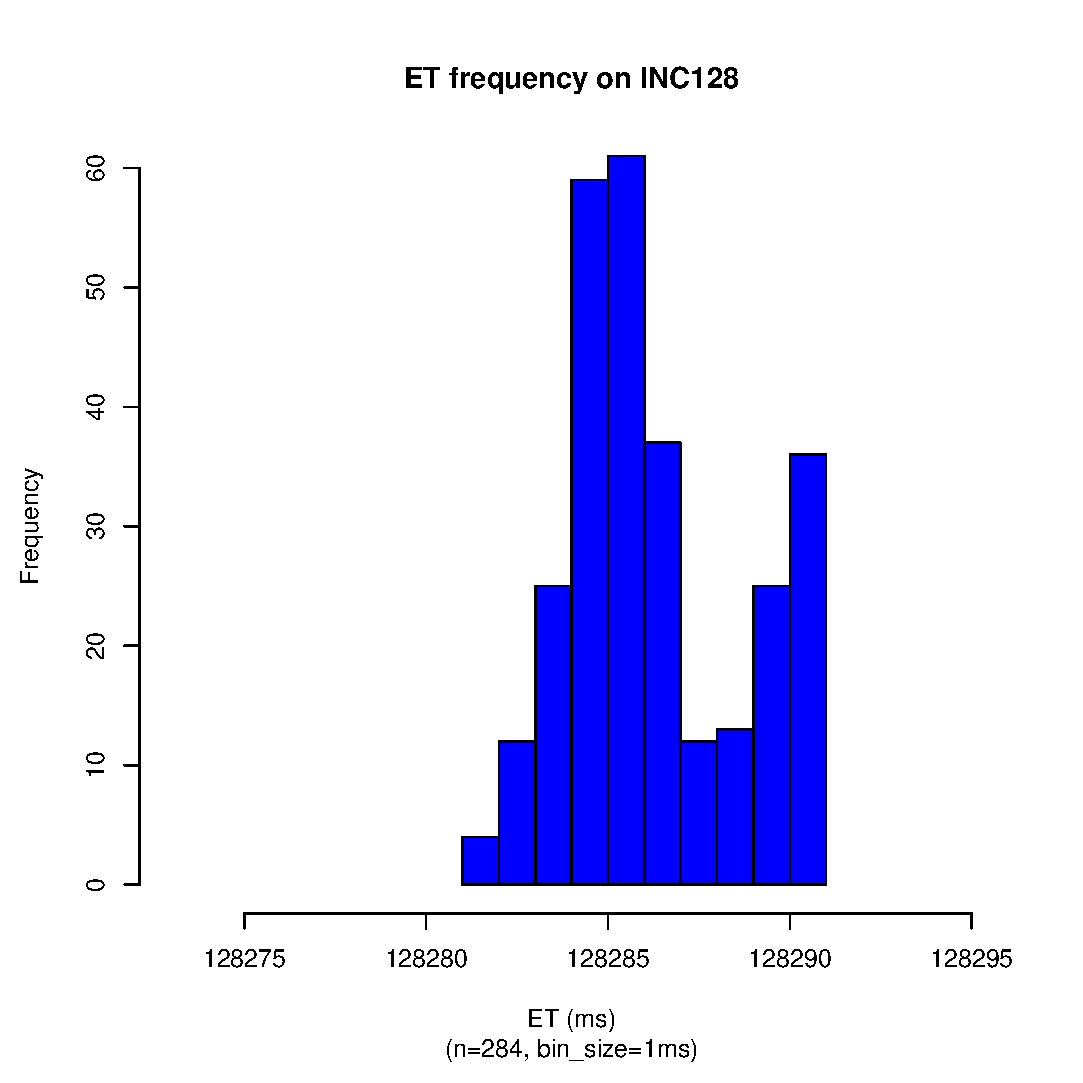
\includegraphics[scale=0.43]{sodb9/128_sec_et_hist_v5.eps}
		\label{fig:inc128_et_hist_v5}
	}
	\caption{ET Histograms of INC16 ... INC128~\label{fig:s9_et_hist2}}
\end{figure}

\newpage

\subsection{PT}

\begin{figure}[hp!]
	\centering
	\subfigure[PT frequency on INC1]{
		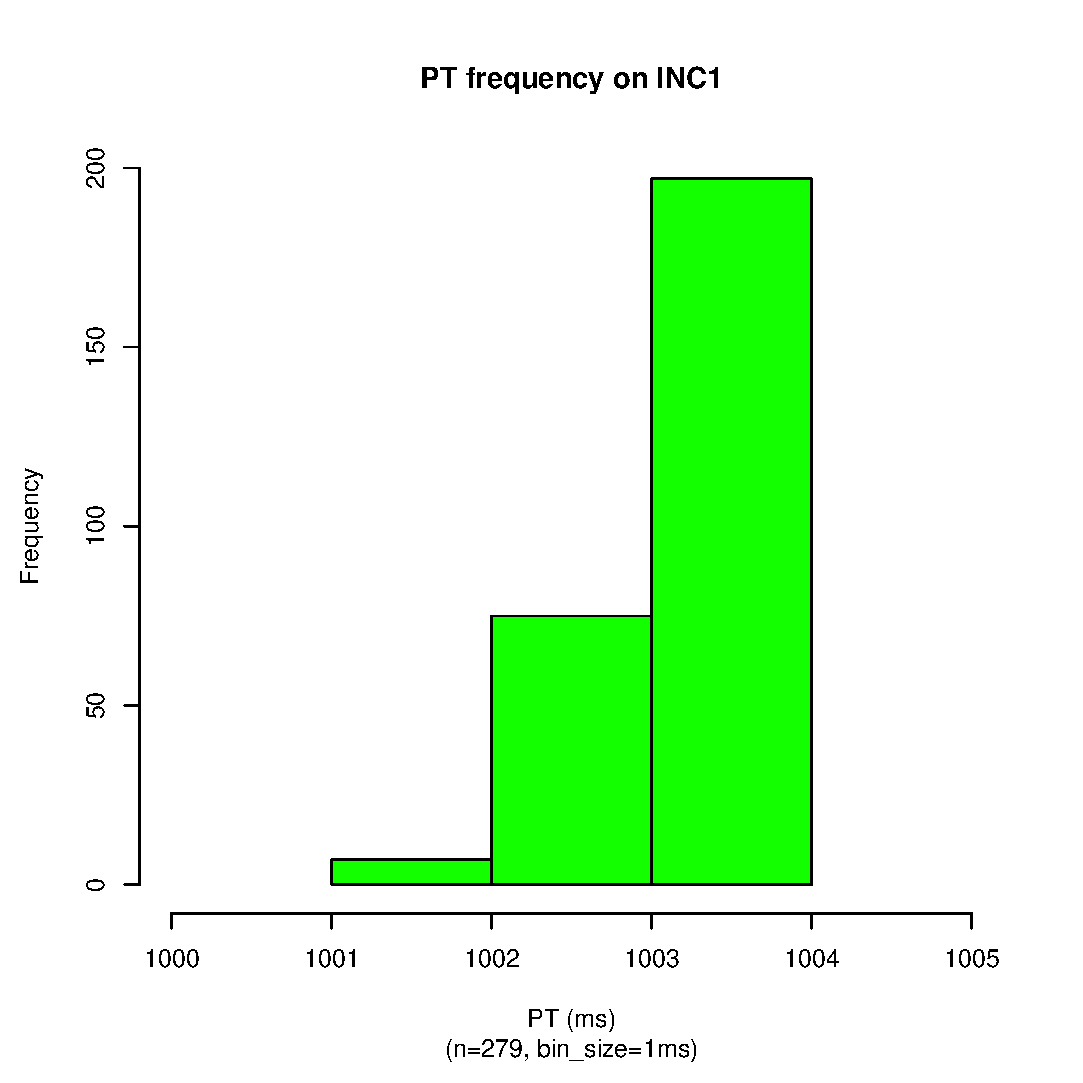
\includegraphics[scale=0.43]{sodb9/1_sec_pt_hist_v5.eps}
		\label{fig:inc1_hist_v5}
	}
	\subfigure[PT frequency on INC2]{
		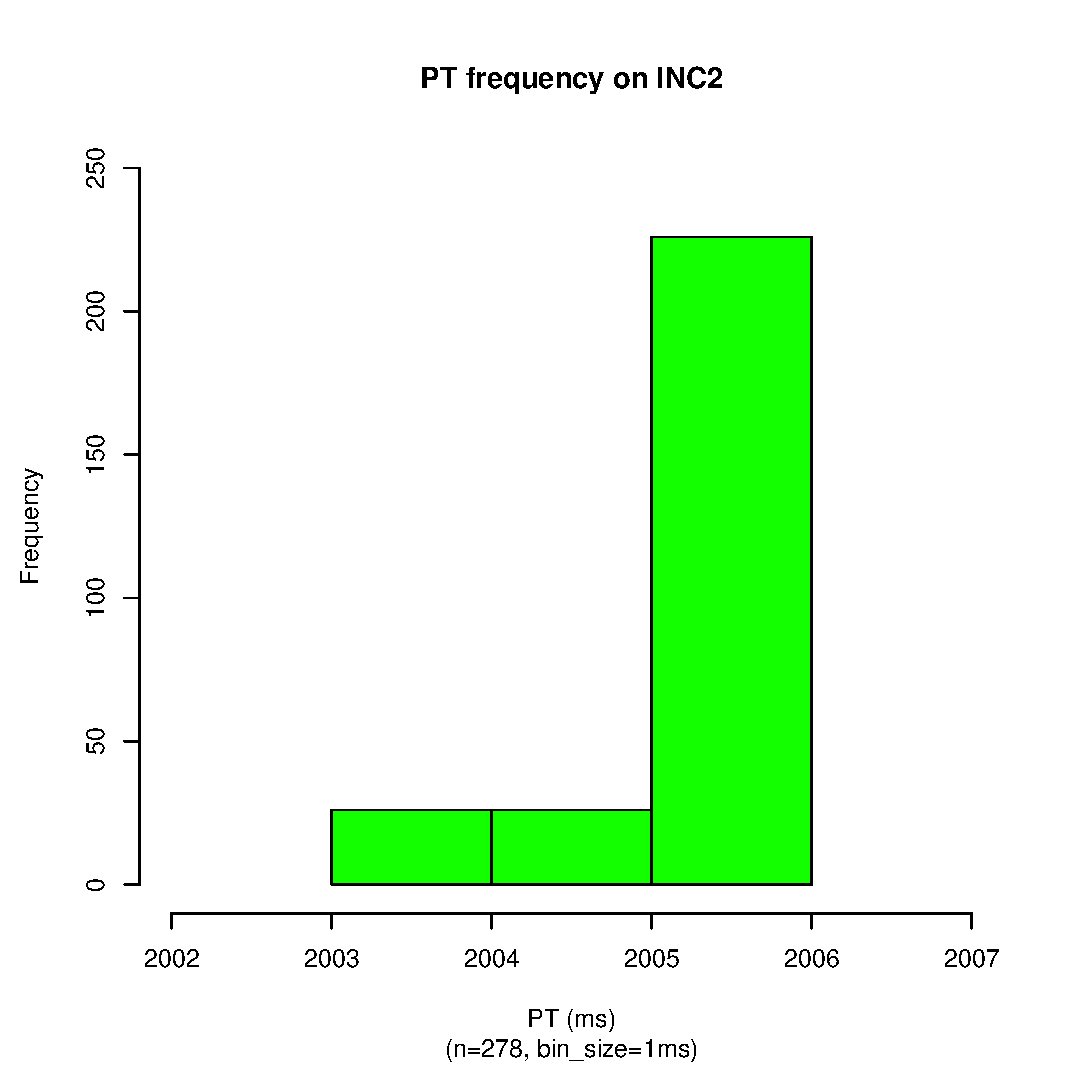
\includegraphics[scale=0.43]{sodb9/2_sec_pt_hist_v5.eps}
		\label{fig:inc2_hist_v5}
	}
	\subfigure[PT frequency on INC4]{
		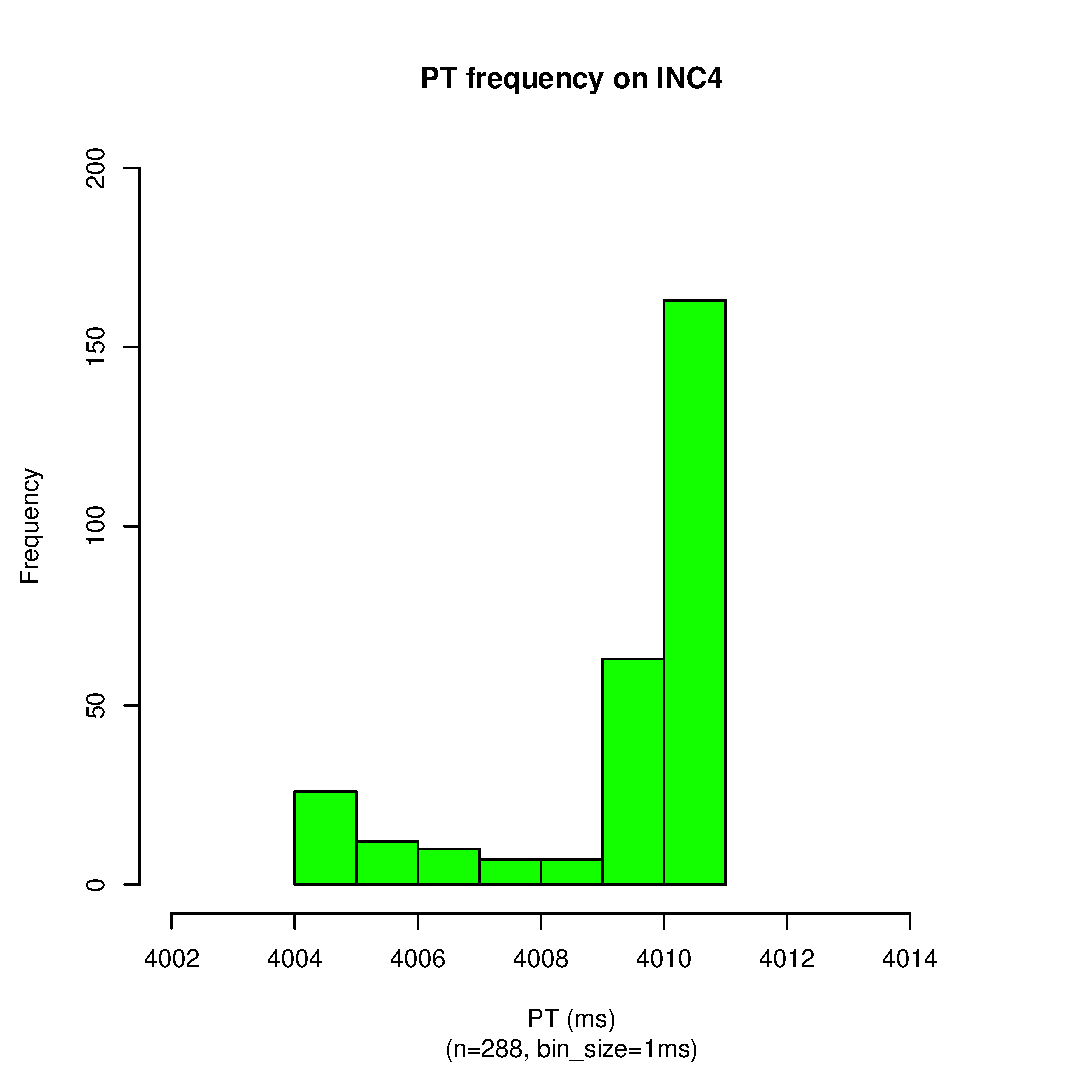
\includegraphics[scale=0.43]{sodb9/4_sec_pt_hist_v5.eps}
		\label{fig:inc4_hist_v5}
	}
	\subfigure[PT frequency on INC8]{
		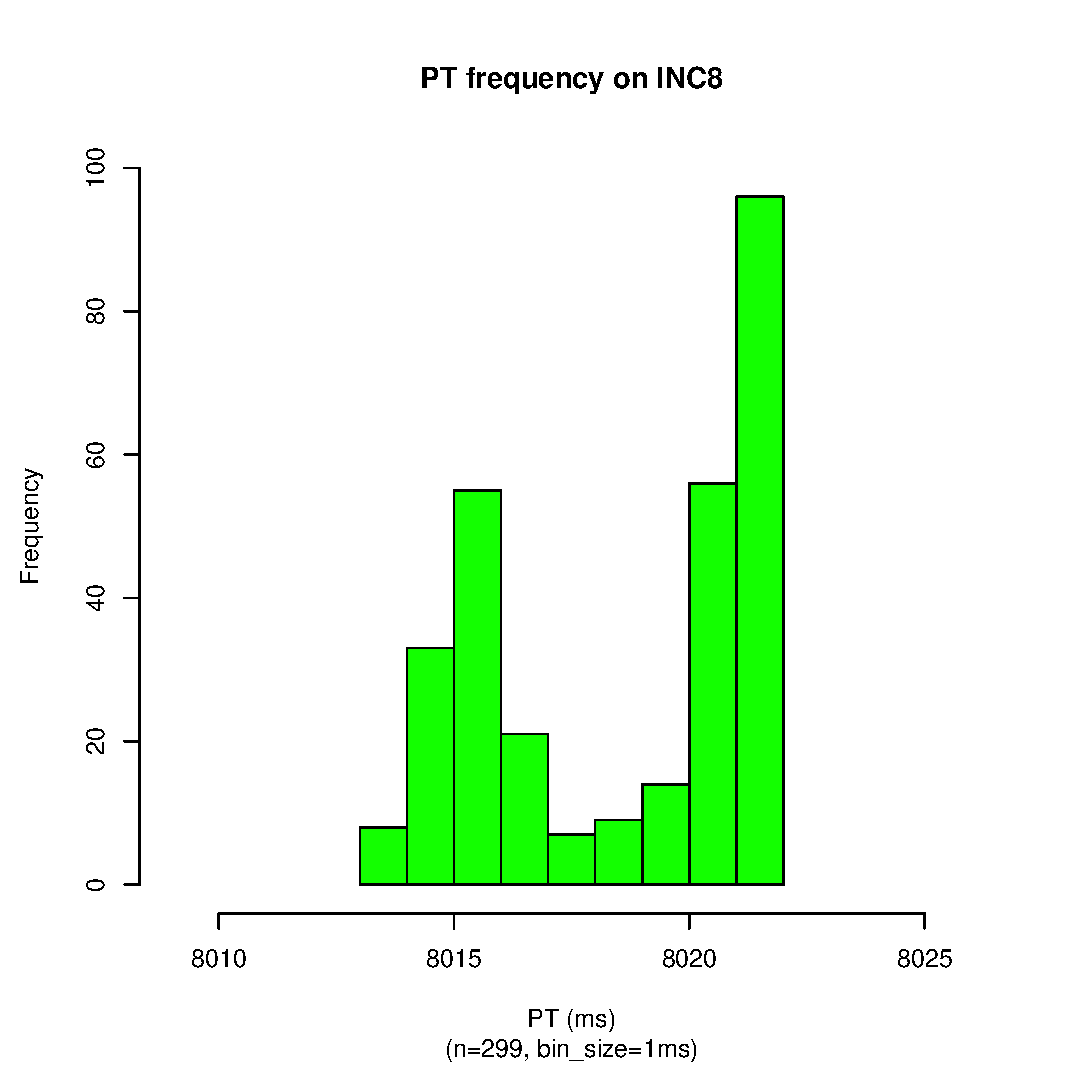
\includegraphics[scale=0.43]{sodb9/8_sec_pt_hist_v5.eps}
		\label{fig:inc8_hist_v5}
	}
	\caption{PT Histograms of INC1 ... INC8~\label{fig:s9_pt_hist1}}
\end{figure}

\begin{figure}[hp!]
	\centering
	\subfigure[PT frequency on INC16]{
		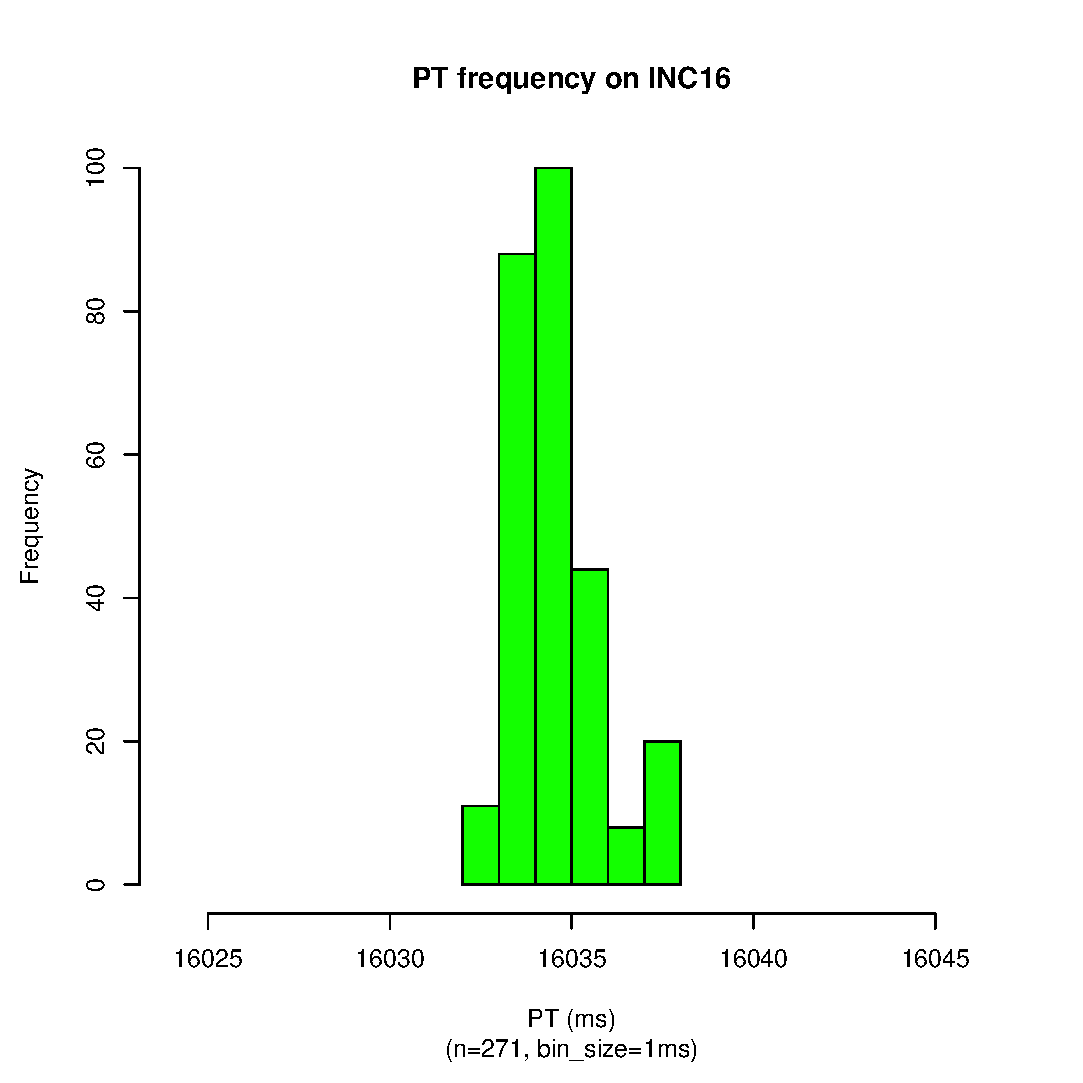
\includegraphics[scale=0.43]{sodb9/16_sec_pt_hist_v5.eps}
		\label{fig:inc16_hist_v5}
	}
	\subfigure[PT frequency on INC32]{
		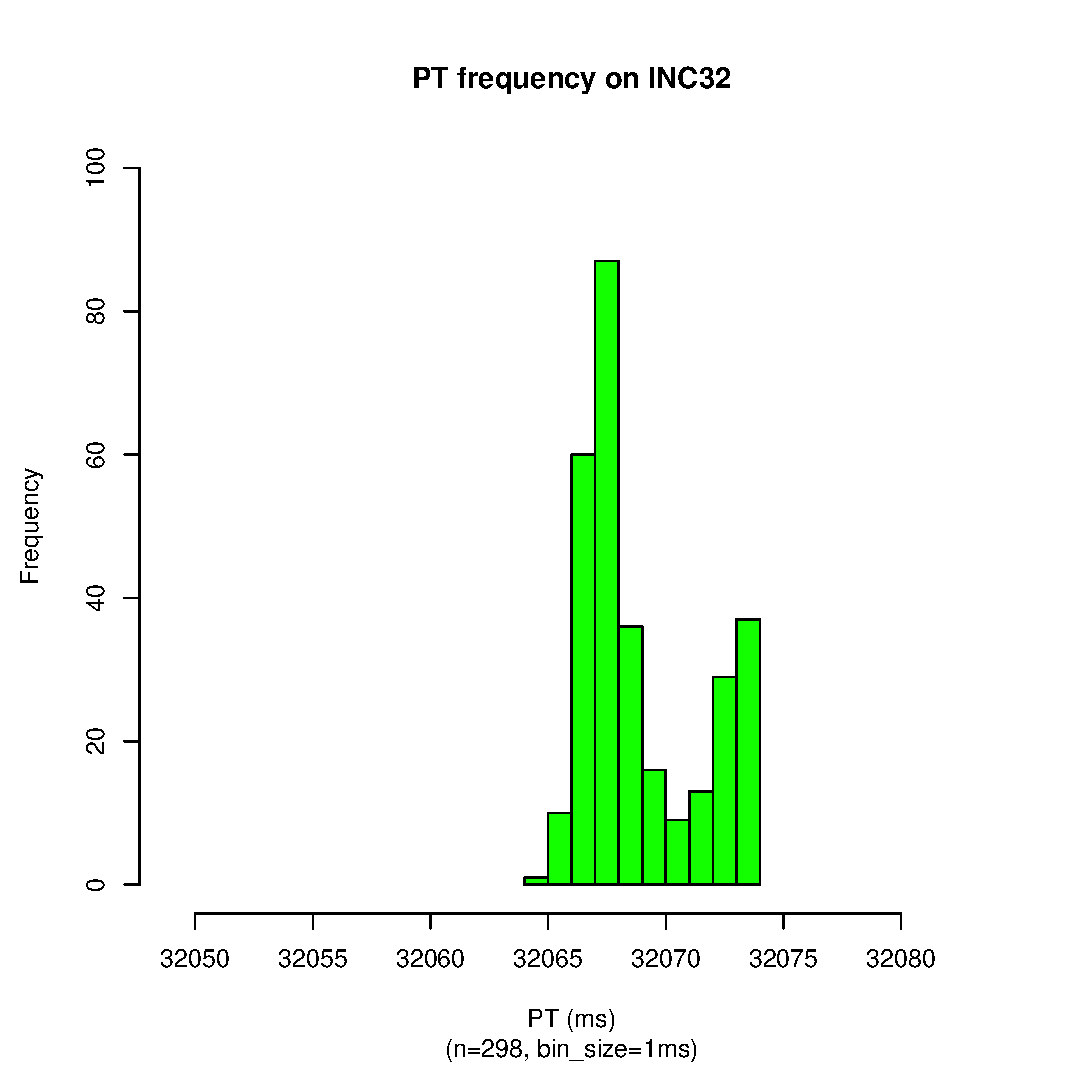
\includegraphics[scale=0.43]{sodb9/32_sec_pt_hist_v5.eps}
		\label{fig:inc32_hist_v5}
	}
	\subfigure[PT frequency on INC64]{
		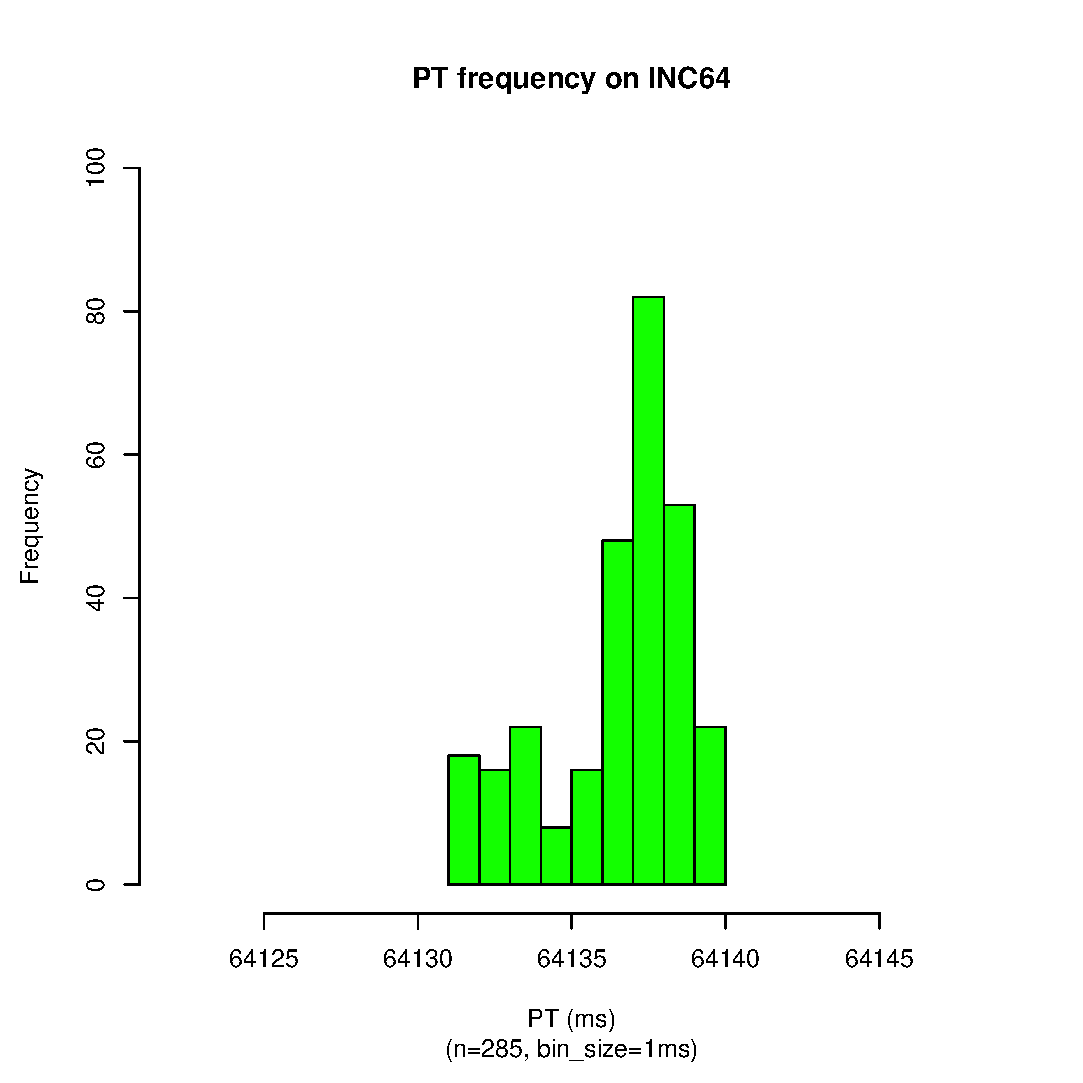
\includegraphics[scale=0.43]{sodb9/64_sec_pt_hist_v5.eps}
		\label{fig:inc64_hist_v5}
	}
	\subfigure[PT frequency on INC128]{
		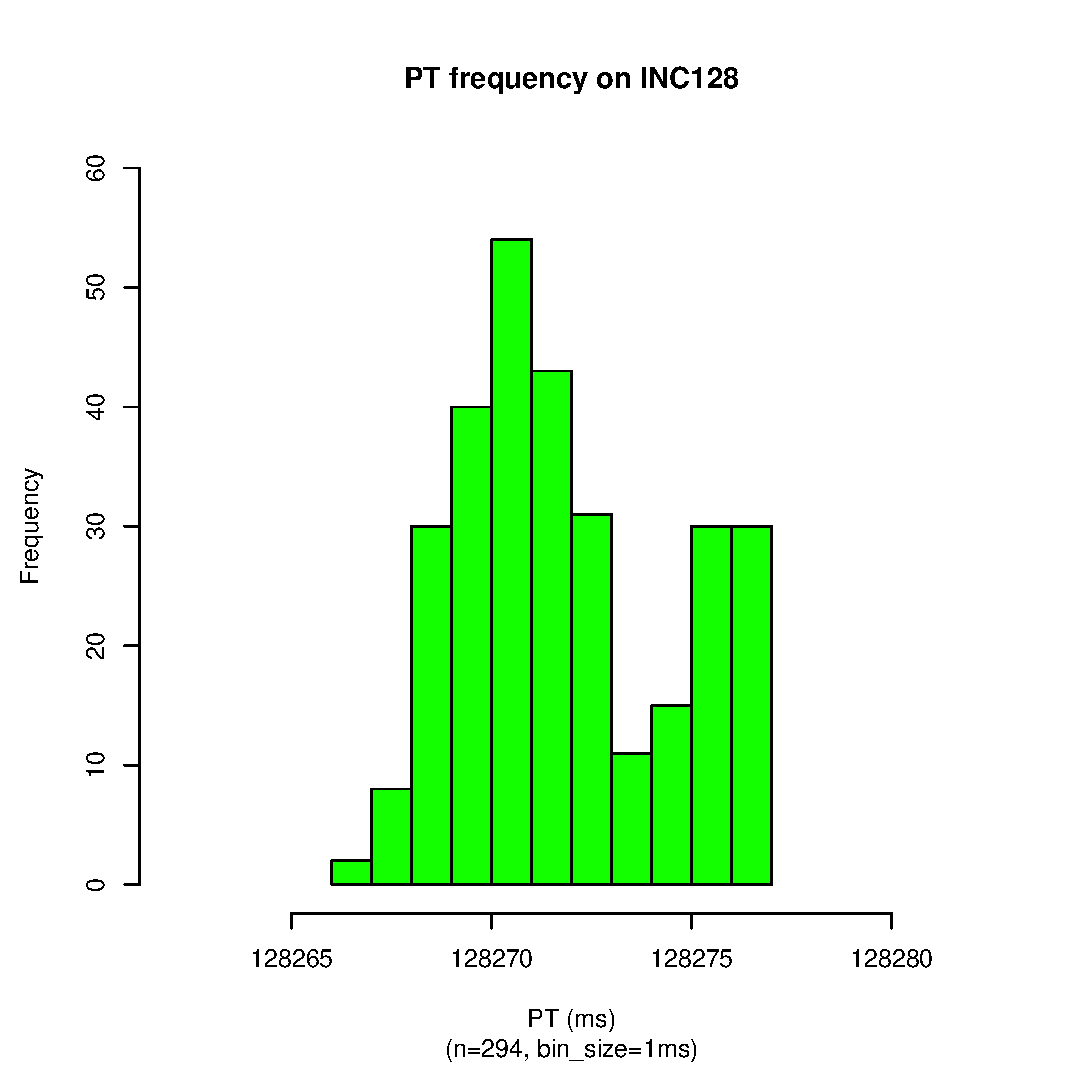
\includegraphics[scale=0.43]{sodb9/128_sec_pt_hist_v5.eps}
		\label{fig:inc128_hist_v5}
	}
	\caption{PT Histograms of INC16 ... INC64~\label{fig:s9_pt_hist2}}
\end{figure}
\newpage

\section{{\tt sodb9}~\label{sec:sodb9_hist}} 
This section exhibits histograms on the EMPv5 data obtained on {\tt sodb9}. 
The detailed description of the base data are from Table~\ref{tab:exp_notes}.

\subsection{ET}

\begin{figure}[hp!]
	\centering
	\subfigure[ET frequency on INC1]{
		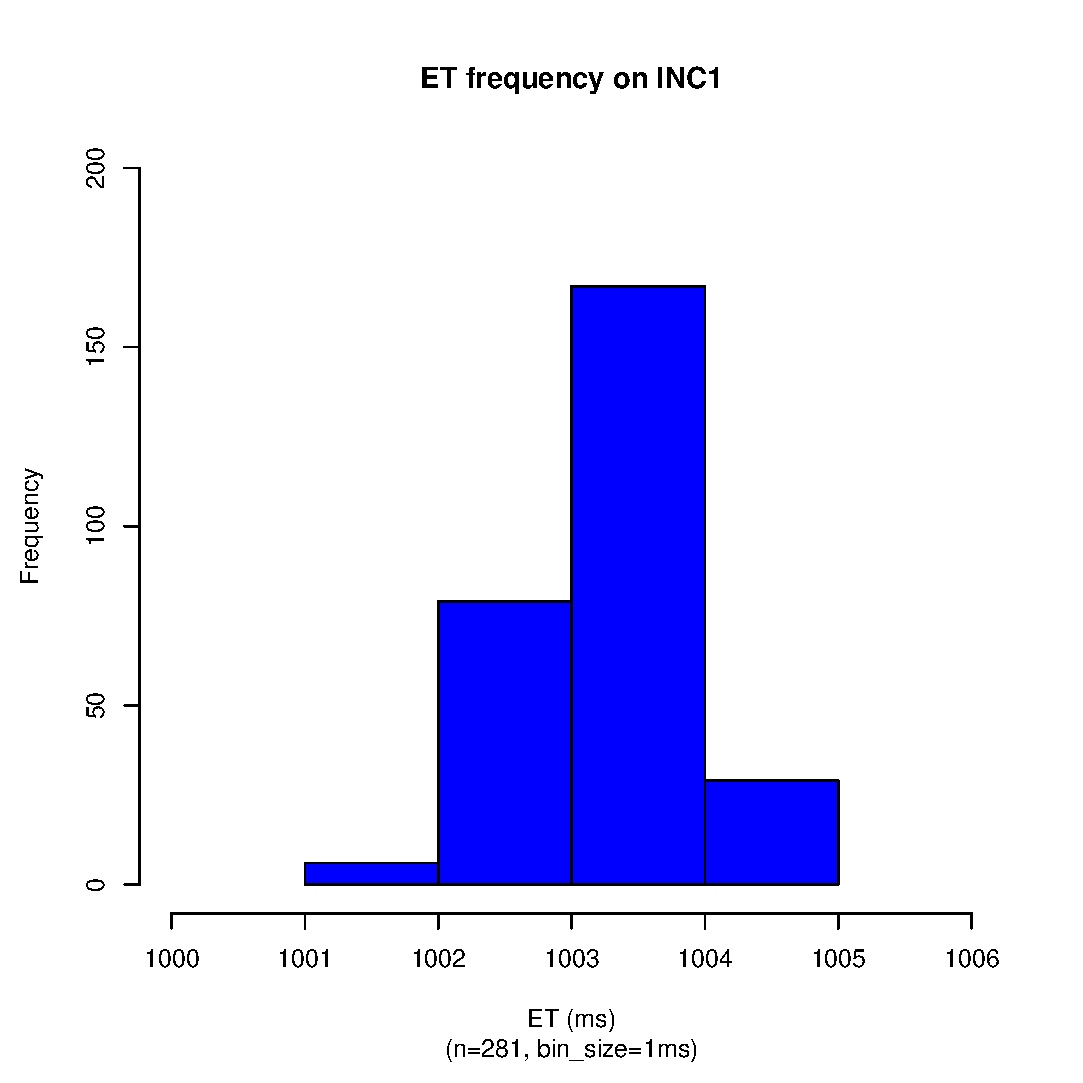
\includegraphics[scale=0.43]{sodb9/1_sec_et_hist_v5.eps}
		\label{fig:inc1_et_hist_v5}
	}
	\subfigure[ET frequency on INC2]{
		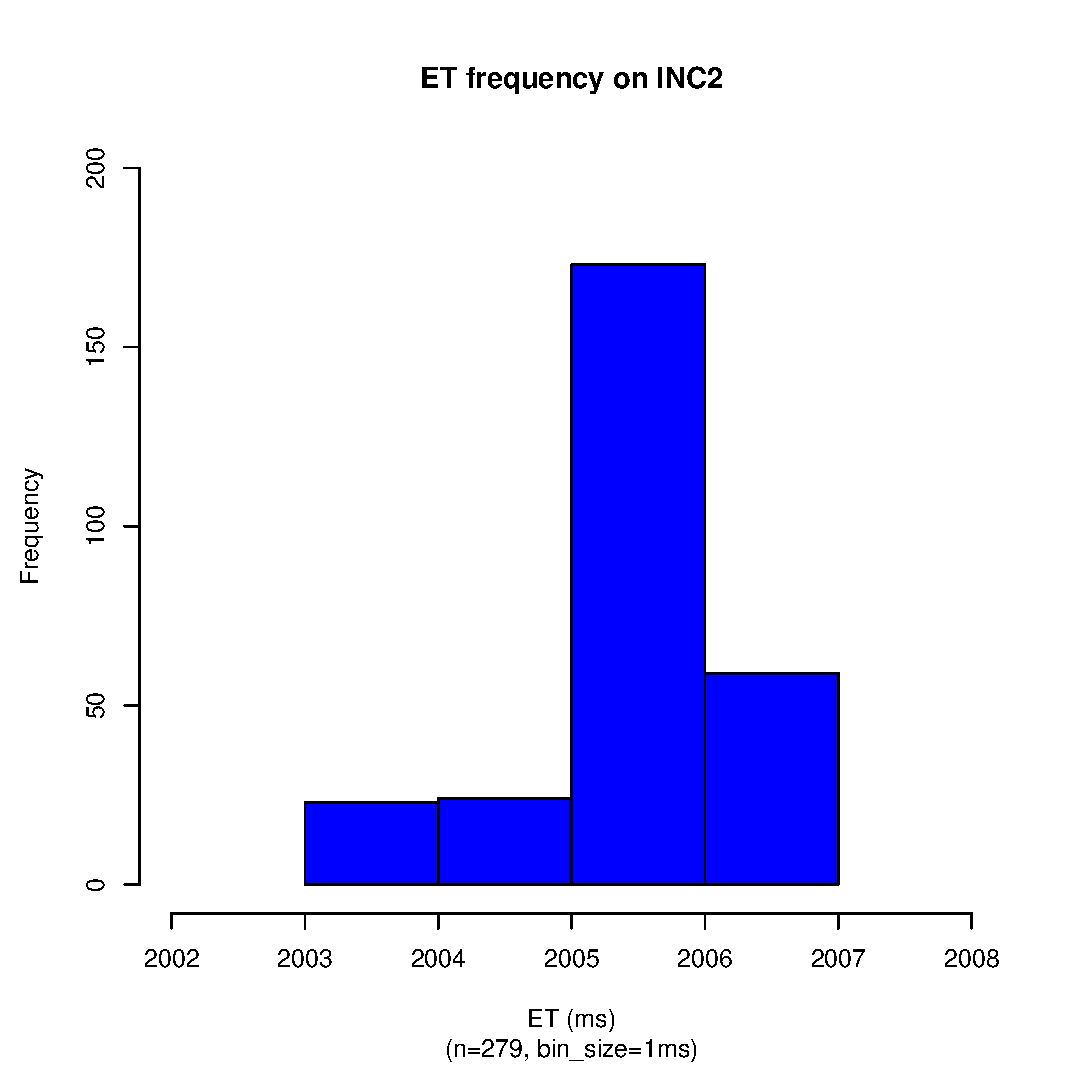
\includegraphics[scale=0.43]{sodb9/2_sec_et_hist_v5.eps}
		\label{fig:inc2_et_hist_v5}
	}
	\subfigure[ET frequency on INC4]{
		\includegraphics[scale=0.43]{sodb9/4_sec_et_hist_v5.eps}
		\label{fig:inc4_et_hist_v5}
	}
	\subfigure[ET frequency on INC8]{
		\includegraphics[scale=0.43]{sodb9/8_sec_et_hist_v5.eps}
		\label{fig:inc8_et_hist_v5}
	}
	\caption{ET Histograms of INC1 ... INC8~\label{fig:s9_et_hist1}}
\end{figure}

\begin{figure}[hp!]
	\centering
	\subfigure[ET frequency on INC16]{
		\includegraphics[scale=0.43]{sodb9/16_sec_et_hist_v5.eps}
		\label{fig:inc16_et_hist_v5}
	}
	\subfigure[ET frequency on INC32]{
		\includegraphics[scale=0.43]{sodb9/32_sec_et_hist_v5.eps}
		\label{fig:inc32_et_hist_v5}
	}
	\subfigure[ET frequency on INC64]{
		\includegraphics[scale=0.43]{sodb9/64_sec_et_hist_v5.eps}
		\label{fig:inc64_et_hist_v5}
	}
	\subfigure[ET frequency on INC128]{
		\includegraphics[scale=0.43]{sodb9/128_sec_et_hist_v5.eps}
		\label{fig:inc128_et_hist_v5}
	}
	\caption{ET Histograms of INC16 ... INC128~\label{fig:s9_et_hist2}}
\end{figure}

\newpage

\subsection{PT}

\begin{figure}[hp!]
	\centering
	\subfigure[PT frequency on INC1]{
		\includegraphics[scale=0.43]{sodb9/1_sec_pt_hist_v5.eps}
		\label{fig:inc1_hist_v5}
	}
	\subfigure[PT frequency on INC2]{
		\includegraphics[scale=0.43]{sodb9/2_sec_pt_hist_v5.eps}
		\label{fig:inc2_hist_v5}
	}
	\subfigure[PT frequency on INC4]{
		\includegraphics[scale=0.43]{sodb9/4_sec_pt_hist_v5.eps}
		\label{fig:inc4_hist_v5}
	}
	\subfigure[PT frequency on INC8]{
		\includegraphics[scale=0.43]{sodb9/8_sec_pt_hist_v5.eps}
		\label{fig:inc8_hist_v5}
	}
	\caption{PT Histograms of INC1 ... INC8~\label{fig:s9_pt_hist1}}
\end{figure}

\begin{figure}[hp!]
	\centering
	\subfigure[PT frequency on INC16]{
		\includegraphics[scale=0.43]{sodb9/16_sec_pt_hist_v5.eps}
		\label{fig:inc16_hist_v5}
	}
	\subfigure[PT frequency on INC32]{
		\includegraphics[scale=0.43]{sodb9/32_sec_pt_hist_v5.eps}
		\label{fig:inc32_hist_v5}
	}
	\subfigure[PT frequency on INC64]{
		\includegraphics[scale=0.43]{sodb9/64_sec_pt_hist_v5.eps}
		\label{fig:inc64_hist_v5}
	}
	\subfigure[PT frequency on INC128]{
		\includegraphics[scale=0.43]{sodb9/128_sec_pt_hist_v5.eps}
		\label{fig:inc128_hist_v5}
	}
	\caption{PT Histograms of INC16 ... INC64~\label{fig:s9_pt_hist2}}
\end{figure}

\end{document}